\documentclass[12pt,oneside]{book}
\usepackage{lmodern}
\usepackage{amssymb,amsmath}
\usepackage{ifxetex,ifluatex}
\usepackage{fixltx2e} % provides \textsubscript
\ifnum 0\ifxetex 1\fi\ifluatex 1\fi=0 % if pdftex
  \usepackage[T1]{fontenc}
  \usepackage[utf8]{inputenc}
\else % if luatex or xelatex
  \ifxetex
    \usepackage{mathspec}
  \else
    \usepackage{fontspec}
  \fi
  \defaultfontfeatures{Ligatures=TeX,Scale=MatchLowercase}
    \setmainfont[]{Georgia}
\fi
% use upquote if available, for straight quotes in verbatim environments
\IfFileExists{upquote.sty}{\usepackage{upquote}}{}
% use microtype if available
\IfFileExists{microtype.sty}{%
\usepackage{microtype}
\UseMicrotypeSet[protrusion]{basicmath} % disable protrusion for tt fonts
}{}
\usepackage[left=1in,right=2in,top=1in,bottom=1in,marginparwidth=1.5in]{geometry}
\usepackage{hyperref}
\hypersetup{unicode=true,
            pdftitle={Prepositional phrase attachment ambiguities in declarative and interrogative contexts: Oral reading data},
            pdfauthor={Tyler J. Peckenpaugh},
            pdfborder={0 0 0},
            breaklinks=true}
\urlstyle{same}  % don't use monospace font for urls
\usepackage{longtable,booktabs}
\usepackage{graphicx,grffile}
\makeatletter
\def\maxwidth{\ifdim\Gin@nat@width>\linewidth\linewidth\else\Gin@nat@width\fi}
\def\maxheight{\ifdim\Gin@nat@height>\textheight\textheight\else\Gin@nat@height\fi}
\makeatother
% Scale images if necessary, so that they will not overflow the page
% margins by default, and it is still possible to overwrite the defaults
% using explicit options in \includegraphics[width, height, ...]{}
\setkeys{Gin}{width=\maxwidth,height=\maxheight,keepaspectratio}
\IfFileExists{parskip.sty}{%
\usepackage{parskip}
}{% else
\setlength{\parindent}{0pt}
\setlength{\parskip}{6pt plus 2pt minus 1pt}
}
\setlength{\emergencystretch}{3em}  % prevent overfull lines
\providecommand{\tightlist}{%
  \setlength{\itemsep}{0pt}\setlength{\parskip}{0pt}}
\setcounter{secnumdepth}{5}
% Redefines (sub)paragraphs to behave more like sections
\ifx\paragraph\undefined\else
\let\oldparagraph\paragraph
\renewcommand{\paragraph}[1]{\oldparagraph{#1}\mbox{}}
\fi
\ifx\subparagraph\undefined\else
\let\oldsubparagraph\subparagraph
\renewcommand{\subparagraph}[1]{\oldsubparagraph{#1}\mbox{}}
\fi

%%% Use protect on footnotes to avoid problems with footnotes in titles
\let\rmarkdownfootnote\footnote%
\def\footnote{\protect\rmarkdownfootnote}

%%% Change title format to be more compact
\usepackage{titling}

% Create subtitle command for use in maketitle
\providecommand{\subtitle}[1]{
  \posttitle{
    \begin{center}\large#1\end{center}
    }
}

\setlength{\droptitle}{-2em}

  \title{Prepositional phrase attachment ambiguities in declarative and interrogative contexts: Oral reading data}
    \pretitle{\vspace{\droptitle}\centering\huge}
  \posttitle{\par}
    \author{Tyler J. Peckenpaugh}
    \preauthor{\centering\large\emph}
  \postauthor{\par}
      \predate{\centering\large\emph}
  \postdate{\par}
    \date{2019-08-19}

\newenvironment{note}
    {\begin{center}
    \begin{tabular}{|p{0.9\textwidth}|}
    \hline
    \singlespacing\\
    }
    { 
    \\\\\hline
    \end{tabular} 
    \end{center}
    }
    
\makeatletter
\preto\@marginparreset{\singlespacing}
\makeatother

\usepackage[commentmarkup=margin,draft]{changes}

\pagenumbering{roman}


\definecolor{dgreen}{RGB}{10,200,120}
\usepackage{booktabs}
\usepackage{longtable}
\usepackage{array}
\usepackage{multirow}
\usepackage{wrapfig}
\usepackage{float}
\usepackage{colortbl}
\usepackage{pdflscape}
\usepackage{tabu}
\usepackage{threeparttable}
\usepackage{threeparttablex}
\usepackage[normalem]{ulem}
\usepackage{makecell}
\usepackage{xcolor}

\usepackage[linguistics]{forest}
\usepackage{longtable}
\usepackage{booktabs}
\usepackage{setspace}\doublespacing

\begin{document}
\maketitle

{
\setcounter{tocdepth}{1}
\tableofcontents
}
\listoftables
\listoffigures
\pagebreak

\raggedright

\hypertarget{abstract}{%
\chapter*{Abstract}\label{abstract}}
\addcontentsline{toc}{chapter}{Abstract}

\emph{Abstract is a work in progress.} This paper reports a study on the effect of interrogativity on the oral reading of temporarily ambiguous prepositional phrases (PPs). Specifically, it looks at sentences ending in a of two PPs, where the first is interpretable as the goal argument of the preceding verb, and the status of the second (PP2 Status) is manipulated to either necessarily be the goal argument of that verb (Arg), forcing reanalysis, or not (Mod), allowing the original parse to stand. No evidence is found that interrogativity impacts the difficulty of understanding the Arg-type sentences, despite an intuitive decrease in difficulty when those sentences are presented in an interrogative context. A double-reading protocol is employed, where participants are asked to read a sentence first without preview (Reading 1), and then after unlimited preview (Reading 2).A robust effect of PP2 Status is found for the prosodic phrasing of the target sentences, and an effect of interrogativity on the study time between Readings, Inter-Reading Time (IRT), is reported.

\hypertarget{acknowledgements}{%
\chapter*{Acknowledgements}\label{acknowledgements}}
\addcontentsline{toc}{chapter}{Acknowledgements}

TBD

\hypertarget{about-this-draft}{%
\section*{About this draft}\label{about-this-draft}}
\addcontentsline{toc}{section}{About this draft}

This represents the document that will be defended on August 29th. The goal is to deposit before September 16, after incorporating whatever revisions are requested.

\pagebreak

\pagenumbering{arabic}
\definechangesauthor[color=brown]{JDF}

\hypertarget{introduction-and-background}{%
\chapter{Introduction and background}\label{introduction-and-background}}

\comment{This paragraph was \P 1 chapter 1}

This paper presents a study on human sentence processing, or parsing, and on the parsing of a particular sort of ambiguity. Parsing is assumed to be the projection of structure by a reader or listener over a string (which obviously lacks inherent structure). Following the sort of model of parsing put forward by, e.g., Kimball (1973), Frazier \& Fodor (1978), and Frazier \& Clifton (1996), this study assumes that parsing is done online and that most material must be incorporated into the structure being built as soon as it is encountered. This can lead to mis-parses, where the parser has guessed wrong about how to incorporate a given phrase with a temporarily ambiguous structure, and then encounters material that cannot be incorporated into the current structure. When this happens, the parser must \replaced{reanalyze the material that had so far been processed, in order to come upa structure that can accomodate both the new and old material grammatically}{discard part or all of its pending structure and try again to incorporate the material encountered so far}. This sort of parser crash is \deleted[id=JDF]{often} called a garden path.

\comment{From here until next note, was introductory section of chapter 2}

\deleted{As briefly mentioned earlier, }``\replaced{G}{g}arden path effects'' occur when a temporarily ambiguous sentence resolves in such a way that the structure initially preferred by the parser is incompatible with how the sentence actually continues. These parsing errors have traditionally been attributed to structurally-focused parsing preferences (Frazier, 1979; Frazier \& Fodor, 1978; Kimball, 1973) that ignore semantic content on the first pass. Frazier (1979) formulates several of these, including the following two which are widely accepted in one form or another:

\begin{enumerate}
\def\labelenumi{(\arabic{enumi})}
\item
  \emph{Minimal attachment}
  Attach incoming material into the phrase-marker being constructed using the fewest nodes consistent with the well-formedness rules of the language under analysis (Frazier, 1979, p. 24)
\item
  \emph{Late closure}
  When possible, attach incoming material into the clause currently being parse\added[id=JDF]{d} (Frazier, 1979, p. 20)
\end{enumerate}

Because these strategies ignore semantic and pragmatic plausibility and the parser typically does not know what material might be further on in the string, mis-parses at temporarily ambiguous regions can occur, resulting in garden paths. \emph{Minimal Attachment} \added[id=JDF]{(MA)} is important to this study and will be revisited later on.

An example is the commonly studied garden path sentence, ``The horse raced past the barn fell'' (Bever, 1970). Here, the initial parse incorrectly assumes that the matrix subject is the unmodified NP the horse, per Minimal Attachment, and takes the matrix verb to be raced, as in the sentence, ``The horse raced past the finish line.''

\begin{enumerate}
\def\labelenumi{(\arabic{enumi})}
\setcounter{enumi}{2}
\tightlist
\item
  The horse raced past the barn fell (Bever, 1970)

  \begin{enumerate}
  \def\labelenumii{\alph{enumii})}
  \tightlist
  \item
    {[}\textsubscript{S} {[}\textsubscript{NP} The horse{]} {[}\textsubscript{VP} raced past the barn{]}{]}   ???   {[}\textsubscript{VP} fell{]}
  \item
    {[}\textsubscript{S} {[}\textsubscript{NP} The horse raced past the barn{]} {[}\textsubscript{VP} fell{]}{]}
  \end{enumerate}
\end{enumerate}

An attempted parse resulting in structure (3 a) crashes, as it is not possible to incorporate the final word fell in a grammatical way. Reanalysis is required, with the grammatical parse being (3 b) where the matrix subject is \emph{the horse raced past the barn}, a noun phrase (NP) containing a reduced relative clause \emph{raced past the barn}. Thus \emph{fell} can be incorporated as the matrix verb, with a structure comparable to, ``The horse (that was) raced past the barn was hungry.''

\deleted{There is an ongoing debate in the literature about what parsing model best fits the empirical facts. This study follows [@frazier1996construal] in assuming that structure-first parsing strategies are at play, in addition to a primary vs. non-primary relation distinction that determines how immediately a phrase must be incorporated into a parse, allowing for some material to be incorporated later and thereby make use of additional information that is not available for immediate parsing decisions.}

\comment{Back to what was chapter 1, $\P$ 2}

The study being reported is concerned with certain sentences that contain \deleted{such} a temporarily ambiguous prepositional phrase (PP1), followed by another \deleted[id=JDF]{PP} (PP2) which \replaced{causes the expected parse to crash}{interferes with what is assumed to be the default interpretation of PP1} \added{Specifically, it is expected that PP1 in} (4) \added{will initially be interpreted as the goal of \em{cram}, but that parse will fail when it is realized that PP2 cannot plausibly modify \em{drawer}.}

\comment{examples moved up slightly}

\begin{enumerate}
\def\labelenumi{(\arabic{enumi})}
\setcounter{enumi}{3}
\item
  He had planned to cram the paperwork {[}\textsubscript{PP1} in the drawer{]} {[}\textsubscript{PP2} in\deleted{to} his briefcase{]}.
\item
  He had planned to cram the paperwork {[}\textsubscript{PP1} in the drawer \deleted{]} {[}\textsubscript{PP2} of his filing cabinet{]}\added{]}.
\end{enumerate}

\added{This contrasts with the similar sentence in} (5) \replaced{where PP2 can plausibly modify *drawer* and so the parse where *in the drawer* is the goal argument is accepted and *of his filing cabinet* is incoporated as a modifier within PP1.}{: as an argument of the verb. The reasons for that assumption are discussed in Section \\ref{mech}, but for now it suffices to understand that (@cramiGPy) represents a difficult to comprehend sentence (a garden path), while (@cramiGPn) presents no such difficulty.}

((examples were here))

\deleted{Before the details of the current research can be outlined, it is first necessary to explain some of the terms and mechanisms involved. This chapter is concerned with doing so.}

\textbackslash{}begin\{note\}
Sections 1.1 and 1.2 are redundant and have been removed. They are incorporated into the above.
\textbackslash{}end

\hypertarget{obs}{%
\section{Motivations for the current}\label{obs}}

\comment{Adapted from what was \S 1.3}

\added{The current study was initially motivated by an observation discovered by Janet Dean Fodor and Dianne Bradley, and originally reported in @qp2. That observation is that a garden path sentence like} (4) \added{repeated here as} (6) \added{is, for whatever reason, not as difficult to process when presented as an interrogative, as in} (7), \replaced{rather than a declarative.}{These attachment ambiguities which are difficult to parse in the declarative, appear to be less difficult to parse when presented in polar interrogative context. Consider again the somewhat difficult to process sentence in (@cramiGPy), repeated below as (@dec) for convenience.}

\begin{enumerate}
\def\labelenumi{(\arabic{enumi})}
\setcounter{enumi}{5}
\item
  He had planned to cram the paperwork {[}\textsubscript{PP1} in the drawer{]} {[}\textsubscript{PP2} in\deleted{to} his briefcase{]}.
\item
  Had he planned to cram the paperwork {[}\textsubscript{PP1} in the drawer{]} {[}\textsubscript{PP2} in\deleted{to} his briefcase{]}?
\end{enumerate}

Peckenpaugh (2016) \added{attempted to find a behavioral correlate of this intuition by looking at variation in reading time of sentence like} (6) and (7), \added{but the results were inconclusive. The current study continues that line of research by looking at similar sentences, while also attempting to control additional factors that may have led to} Peckenpaugh (2016)'s \added{inconclusive results. One such concern is that} (6) \added{relies on the implausibility of a drawer within a briefcase, i.e., real world knowledge, in order to disambiguated the appropriate attachment sites for PP1 and PP2. Real world knowledge and beliefs of what is or is not plausible varies between speakers and may not always be reliable as a trigger for reanalysis. The current study makes use of carefully constructed sentences (the criteria by which they were constructed is detailed in Section} \ref{mat}\added{) which do not rely on plausibility or pragmatics to disambiguated the PP attachment sites, but instead make use of syntactic disambiguation by including a PP2 that cannot grammatically be incorporated into PP1, as in} (8).

\begin{enumerate}
\def\labelenumi{(\arabic{enumi})}
\setcounter{enumi}{7}
\tightlist
\item
  He had planned to cram the paperwork {[}\textsubscript{PP1} in the drawer{]} {[}\textsubscript{PP2} \emph{into} his briefcase{]}.
\end{enumerate}

\added{The change from pragmatically disambiguation to syntactic disambiguation creates an important distinction between the original observation in} Peckenpaugh (2016) \added{and what the current study is considering. It cannot be assumed that the intuition about} (6) vs.~(7) \added{necessarily extends to cases like} (8), \added{and so one of the questions the current study asks is whether the intuition can be shown to extend to syntactically disambiguated cases that are similar to the pragmatically disambiguated cases for which the observation was first made. In order to keep clear this fine but important difference, a convention is adopted throughout this document where the intuited amelioration of the garden path effect in pragmatically disambiguated cases is referred to as the 2016 intuition, while the possiblity that the intuition extends to syntactically disambiguated cases is referred to as the current hypothesis.}

\comment{these are new to this chapter, but are taken from the discussion chapter, where we discussed them on 8/16}

\begin{enumerate}
\def\labelenumi{(\arabic{enumi})}
\setcounter{enumi}{8}
\item
  \emph{The \added{2016} intuition:} Certain pragmatically disambiguated prepositional phrase (PP) attachment ambiguities which are difficult to parse in the declarative are less difficult to parse when presented as yes-no interrogatives (e.g., Jed crammed the newspapers under the sofa in the trashcan).
\item
  \emph{The current hypothesis:} The intuition may be extensible to PP attachment ambiguities that are syntactically disambiguated in addition to those that are pragmatically disambiguated (e.g., Had he planned to cram the paperwork {[}\textsubscript{PP1} in the drawer{]} {[}\textsubscript{PP2} into his briefcase{]}?).
\end{enumerate}

\deleted{While both sentences contain a temporary ambiguity for the attachment of PPs occurring in string-linear sequence at the end of an utterance, it is more likely in (@intr) that a listener or reader will come away with a plausible interpretation on the first try. This study explores the factors involved in why that is, and seeks to uncover a behavioral correlate of this intuition. If the existence and mechanics of this effect can be pinned down, it will lend insight into what information the parser has access to when making decisions, or when repairing broken parses. This initial observation reveals a robust program of research with many interwoven questions.}

\replaced{In addition to exploring the possible extensibility of the 2016 intuition, the current study is interested in}{One might also ask} what property or properties of polar questions might lead to an easier parsing of garden paths, or at least to the perception that they are easier to parse \replaced{when compared to}{as polar questions than as} declaratives. Because there are minimal differences between the polar question and declarative version of \replaced{declarative versions of these sentences}{a given sentence}, it is \replaced{fairly easy}{reasonable} to assume that the cause lies in one of two domains: the prosodic changes triggered by the use of question intonation, or the pragmatic and semantic properties that are not shared across the versions.

An obvious reflex of the former possibility is another question: how are the various versions of these sentences actually pronounced\added{, prosodically}? \deleted{This question is deceptively difficult to answer;} \replaced{T}{t}he reported study seeks to answer it, but while the recordings collected provide some insight, more work is likely needed to satisfactorily provide an answer.

Likewise, the latter possibility leads one to wonder: what are the semantic and pragmatic differences between a polar question and its declarative counterpart? This question can be approach in a more theoretical way, and has been to some degree in the literature. That said, it remains to be determined how those properties could lead to an easier parsing process, and whether or not a satisfactory explanation for the intuition at large can be pulled from these differences.

\hypertarget{mech}{%
\section{Structural overview of the ambiguity relevant to this study}\label{mech}}

\comment{the following is adapted from what was $\S 2.1$}
\added{The 2016 intuition and the current hypothesis are both concerned with a temporarily ambiguous sequence of PPs at the end of a sentence. This section will discuss what the possible attachment sites for those PPs are and which structures ultimately do and do not work.}

\added{The example in} (11) \added{shows a pragmatically disambiguated sentence with an argument-PP2. The initial parse (a) is implausible, resulting in structural reanalysis to the prefereable parse in (b).}

\begin{enumerate}
\def\labelenumi{(\arabic{enumi})}
\setcounter{enumi}{10}
\tightlist
\item
  Jed crammed the newspapers under the sofa in the \replaced{wastebasket}{trashcan}.
\end{enumerate}

\begin{enumerate}
\def\labelenumi{\alph{enumi})}
\tightlist
\item
  \(\#\) \ldots{} {[}\textsubscript{VP} crammed {[}\textsubscript{NP} the newspapers{]}\\
  {[}\textsubscript{PP1} under {[}\textsubscript{NP} the sofa {[}\textsubscript{PP2} in the wastebasket{]}{]}{]}\\
\item
  \(\checkmark\) \ldots{} {[}\textsubscript{VP} crammed {[}\textsubscript{NP} the newspapers {[}\textsubscript{PP1} under {[}\textsubscript{NP} the sofa {]}{]}
  {[}\textsubscript{PP2} in the \replaced{wastebasket}{trashcan}{]}{]}
  \emph{``\(\#\)'' indicates a structure with an implausible reading}
\end{enumerate}

\replaced{The initial parse is expected to be (a) because of}{In parsing (@aa a), there is} a \deleted{fairly strong} bias (due to \emph{Minimal Attachment}, or some variation thereof), which favors a structure where the first PP attaches into the verb phrase (VP) as an argument of the verb, i.e., {[}\textsubscript{VP} V NP PP1{]}, which leaves nowhere for the second PP to attach but as a modifier of the noun phrase (NP) inside PP1 ({[}\textsubscript{PP1} \emph{under} {[}\textsubscript{NP} \emph{the sofa} {[}\textsubscript{PP2} \emph{in the trashcan}{]}{]}{]}). This initial parse (11 a) is pragmatically implausible, as one does not generally find sofas inside wastebaskets. \added[id=JDF]{Structural} \replaced{r}{R}eanalysis is required to bring about the correct parse (11 b), where PP1 attaches as an NP modifier of the direct object and so allows PP2 to attach as a VP argument, resulting in a structure such as {[}\textsubscript{VP} V {[}\textsubscript{NP} N PP1{]} PP2{]}, i.e., where it is the newspapers under the sofa that are being crammed in the trashcan.

\added{It is important to be clear on how the sentences of concerned are structured. As a matter of terminology, the current study categorizes the sentences being discussed into two groups based on the status of the PP2 they contain: (a) cases where PP2 is an argument are Arg-type sentences, and (b) cases where PP2 is a modifier are Mod-type sentences. In practice, Arg sentences are garden paths, because PP2 must fill the goal role that PP1 is expected to have filled as just discussed. Mod sentences are not garden paths, because PP2 can modify the NP within PP1 and become part of the goal, and therefore need not disrupt PP1 from being the goal.}

\comment{this example has been moved up}

\begin{enumerate}
\def\labelenumi{(\arabic{enumi})}
\setcounter{enumi}{11}
\tightlist
\item
  \textbf{PP2 Status}

  \begin{enumerate}
  \def\labelenumii{(\alph{enumii})}
  \tightlist
  \item
    \emph{PP2 Argument} (Arg) \linebreak
    He had planned to cram the paperwork {[}\textsubscript{PP1} in the drawer{]} {[}\textsubscript{PP2} into his briefcase{]}.
  \item
    \emph{PP2 Modifier} (Mod) \linebreak
    He had planned to cram the paperwork {[}\textsubscript{PP1} in the drawer {[}\textsubscript{PP2} of his filing cabinet{]}{]}.
  \end{enumerate}
\end{enumerate}

In order for the differing parsing process for (12 a) and (12 b) to be explained by a strictly structurally based model of parsing, certain assumptions \deleted{would} have to be made about the syntax. A simple way to get the explanation to work is to assume that all arguments of a verb are syntactic sisters to the verb, resulting in a three-way branching VP for ditransitive verbs. In this case, in order to avoid postulating extra nodes that would be required for PP1 to be a modifier, \emph{Minimal Attachment} dictates that PP1 should be assumed to fill the argument slot. This is not how modern syntactic theory assumes the structure looks, as three-way branching is proscribed. Figures \ref{fig:modTree} and \ref{fig:argTree} show the presumed \deleted{modern} structure\footnote{Note that when the internal structure of an NP is not relevant (no PP is within it) it is not drawn, i.e.~{[}NP newspapers{]} is shorthand for {[}NP {[}N' {[}N newspapers{]}{]}{]}.} of these sentence\deleted{, graphically}.

\begin{figure}[H]
  \centering
  \begin{forest}
    where n children=0{tier=word,font=\normalsize}{}
    \footnotesize
    [\dots
      [VP 
        [V' 
          [V' 
            [V [cram]] 
            [DP 
              [D' 
                [D [the]] 
                [NP [newspapers]]
                ]
              ]
            ]
          ]
          [PP1
            [P' 
              [P [under]] 
              [DP 
                [D'
                  [D [the]] 
                  [NP
                    [N'
                      [N' [N [sofa]]]
                      [PP2$_{Mod}$
                        [P'
                          [P [from]] 
                          [DP 
                            [D' 
                              [D [the]] 
                              [NP [thrift store]]
                            ]
                          ]
                        ]
                      ]
                    ]
                  ]
                ]
              ]
            ]
          ]
        ]
      ]
    ]
  \end{forest}
  \caption{Syntactic tree of an illustrative example sentence with an ambiguous PP1 and a modifier-PP2 (Mod).}
  \label{fig:modTree}
\end{figure}

\begin{figure}
  \centering
  \begin{forest}
    where n children=0{tier=word,font=\normalsize}{}
    \footnotesize
    [\dots
      [VP 
        [V' 
          [V' 
            [V [cram]] 
            [DP 
              [D' 
                [D [the]] 
                [NP 
                  [N' 
                    [N [newspapers]]
                  ] 
                  [PP1 
                    [P'
                      [P [under]] 
                      [DP 
                        [D' 
                          [D [the]] 
                          [NP [sofa]]
                        ]
                      ]
                    ]
                  ]
                ]
              ]
            ]
          ]
          [PP2$_{Arg}$
            [P' 
              [P [into]] 
              [DP 
                [D'
                  [D [the]] 
                  [NP [wastebasket]]
                ]
              ]
            ]
          ]
        ]
      ]
    ]
  \end{forest}
  \caption{Syntactic tree of an illustrative example sentence with an ambiguous PP1 and an argument-PP2 (Arg).}
  \label{fig:argTree}
\end{figure}

\deleted{Note that}\replaced{T}{t}he most pronounced structural difference between the two structures is that in the sentence with a \added{modifier-}PP2 \replaced{(Mod)}{Modifier} the major disjuncture \deleted{, i.e., change in branching direction,} comes \replaced{fairly}{much} earl\replaced{y}{ier}, just after the object NP \emph{the newspapers}. For the \deleted{Arg} sentences with \added{argument-}PP2s \added{(Arg)}, the \replaced{major disjuncture}{branch direction change} is \deleted{much} later, just after PP1 \added{(}\emph{under the sofa}\added{)}.

\deleted{This paper is not interested in the particularities of syntactic theory, and it also is not necessary to rely on *Minimal Attachment* to make the necessary distinction, though it very likely does play a role. Instead, we can focus on distinction added to parsing theory in Construal [@frazier1996construal]: that of primary vs. non-primary relations.}

\deleted{This study is focused on the impact of Speech Act, i.e., where a sentence is interrogative (Q) or declarative (D), in a particular sort of garden path. Specifically, it is concerned with garden path sentences containing a temporary ambiguity that centers on the attachment of two prepositional phrases (PPs) occurring in string-linear sequence at the end of an sentence, e.g., “When we saw her, the nanny had seated the cranky little boy [~PP1~ on the swing] [~PP2~ in his stroller].” }

\replaced{It bears mentioning}{Note} that \emph{Minimal Attachment} as defined by (Frazier, 1979) is somewhat at odds with recent developments in syntactic theory, e.g., obligatory binary branching (cf.~Chomsky, 2014, p. 62). As originally postulated, \emph{Minimal Attachment} \replaced{relies on}{assumes that} a verb with multiple internal arguments incorporat\replaced{es}{ing} each of those arguments as a sister (i.e., a ternary branching structure \comment{new figure: ternary tree} as in \ref{fig:threetree}).

\begin{figure}
  \centering
  \begin{forest}
    where n children=0{tier=word,font=\normalsize}{}
    \footnotesize
    [VP
      [V]
      [DP]
      [PP]
    ]
  \end{forest}
  \caption{Illustrative syntactic tree of a ternary-branching VP.}
  \label{fig:threetree}
\end{figure}

With current theories \added{of syntax} where binary branching is obligatory, two XPs (NP and PP) cannot both be syntactic sisters of the verb, and the structures are assumed to be as shown in the trees presented earlier (Figures \ref{fig:modTree} and \ref{fig:argTree}) so it becomes less clear that the VP attachment site for PP1 actually creates fewer nodes than the lower NP attachment site. Nonetheless, the preference for VP attachment in these kinds of sentences is there, be it due to Minimal Attachment, a preference for arguments over non-arguments, or something else, as evidenced by experimental data from e.g., Rayner, Carlson, \& Frazier (1983) and Clifton, Speer, \& Abney (1991).

\deleted{This study is focused on the impact of Speech Act (interrogative vs. declarative) and its interaction with a trailing sequence of  prepositional phrases (PPs), where the second is of two possible types. The contrasting types of PP2 shown in (@pp2t) are (a) a PP2 which must be an argument, and (b) one which can be a modifier.}

\deleted{PP1, *in the drawer*, is the same in both (@pp2t a) and (@pp2t b), and is ambiguous on first encounter, as it could modify the paperwork or it could be the goal of cram. In (@pp2t a), however, PP2 must ultimately be interpreted as the goal of the verb *cram* because *into his briefcase* cannot modify *the drawer*. Because *cram* only accepts one goal, this means that PP1 in (@pp2t a) has to end up as a modifier of *the paperwork*.  In (@pp2t b), on the other hand, PP2 *of his filing cabinet* can (in this case, must) modify *the drawer*, and so in the drawer can and does end up as the goal of cram. The difference in PP2 Status between (@pp2t a) and (@pp2t b) results in different structures, which I argue are reached by different parsing mechanisms. Namely, (@pp2t a) should, by hypothesis, result in a parse which initially incorporates PP1 as the goal argument of *cram* but then fails and triggers reanalysis when PP2 is encountered. Conversely, (@pp2t b) should by hypothesis allow a straightforward parse where PP1 is initially and ultimately slotted in as the goal of *cram*, since PP2 poses no issue when interpreted as a modifier of *the drawer*. This means (@pp2t b) should not trigger reanalysis. Where (@pp2t a) is a so-called garden path sentence, (@pp2t b) is not. In what follows, I will use the term "argument attachment of PP2" to mean the garden path case, i.e., a sentence that is presumed to require reanalysis, and "modifier attachment of PP2" to mean the straightforwardly parsed case where PP1 is the goal argument.}

\replaced{Rather than worry about}{This paper is not interested in} the particularities of syntactic theory\deleted{,} and \replaced{it also is not necessary to rely on}{the exact formulation of} \emph{Minimal Attachment}, \replaced{an appeal can be made to}{make the necessary distinction, though it very likely does play a role. Instead, we can focus on} \added{a} distinction added to parsing theory in \emph{Construal} (Frazier \& Clifton, 1996): that of primary vs.~non-primary relations. \comment{collapsed two \P into one} \deleted{The impetus behind adding this} \replaced{T}{t}his additional machinery \deleted{to the theory of parsing} is independently motivated: while structure-first decision making seems to hold for the parsing of many structures, there are some that seem to \replaced{follow different rules}{flout them}. \emph{Construal} illustrates this by way of relative clause (RC) attachment in constructions like (13).

\begin{enumerate}
\def\labelenumi{(\arabic{enumi})}
\setcounter{enumi}{12}
\tightlist
\item
  {[}\textsubscript{NP1} The daughter\textsubscript{i}{]} of {[}\textsubscript{NP2} the colonel\textsubscript{j}{]} {[}\textsubscript{RC} who\textsubscript{i/j} was standing on the balcony{]} \ldots{}
\end{enumerate}

The RC in (13) can modify either NP1, the daughter, or NP2 the colonel. A structure-first parsing system, together with the widely agreed upon structural parsing strategy \emph{Late Closure}, \replaced{predict}{would be expected to manifest as} a consistent preference for \deleted[id=JDF]{the} local attachment of the RC in (13), i.e., the structure where the RC modifies NP2. Instead, what \deleted{Frazier and Clifton describe, based on} a number of \added[id=JDF]{empirical} studies (e.g., Clifton, 1988; Cuetos \& Mitchell, 1988) \added{find} is a pattern where the preferred structure depends on the relationship between NP1 and NP2. \deleted{They}Frazier \& Clifton (1996) describe five categories of relationship, and a gradient of preferred RC attachment, from NP1 preference to NP2 preference.

\begin{enumerate}
\def\labelenumi{(\arabic{enumi})}
\setcounter{enumi}{13}
\tightlist
\item
  \textbf{RC Attachment by NP1-NP2 relation} (Frazier \& Clifton, 1996)

  \begin{enumerate}
  \def\labelenumii{\alph{enumii})}
  \tightlist
  \item
    \emph{Material} \linebreak
    The table of wood {[}\textsubscript{RC} that was from Galicia{]}
  \item
    \emph{Quantity} \linebreak
    The glass of wine {[}\textsubscript{RC} you liked{]}
  \item
    \emph{Relational} (friend, enemy, son, and other argument taking NPs, e.g., picture-NPs) \linebreak
    The son of the woman {[}\textsubscript{RC} that was dying{]}
  \item
    \emph{Possessive} \linebreak
    The car of the company {[}\textsubscript{RC} that was falling apart{]}
  \item
    \emph{Non-accompaniment} with \linebreak
    The girl with the hat {[}\textsubscript{RC} that looked funny{]}
  \end{enumerate}
\end{enumerate}

Frazier \& Clifton (1996) \replaced{cite studies showing}{report} that (14 a-b) type configurations favor NP1 RC attachment, (14 e) type configurations favor NP2 RC attachment, while (14 c-d) are intermediate. They argue that this gradient cannot be readily explained by structural parsing, and instead make use of a mechanism they call \deleted{structural} association. RCs, rather than being immediately slotted into a tree in a specific way, are associated with a thematic domain, i.e., the maximal projection of whatever lexical item last assigned theta-roles, together with associated functional projections; in the case of the examples in (14), the last theta assigner is NP2, and its domain extends up to the DP that contains NP1. This is a \replaced{later}{looser} parsing decision that allows the syntactic structure to be decided \deleted{on later,} after semantic information becomes available: the RC can ultimately modify whichever member of the thematic domain is appropriate.

The crucial issue that distinguishes cases where structural association vs.~structural parsing is appropriate is the idea of primary vs.~non-primary relations. Frazier and Clifton formalize this distinction as (15).

\comment[id=JDF]{citation moved and quotation marks added to show this is a direct quote}

\begin{enumerate}
\def\labelenumi{(\arabic{enumi})}
\setcounter{enumi}{14}
\tightlist
\item
  "Primary phrases and relations include

  \begin{enumerate}
  \def\labelenumii{\alph{enumii})}
  \tightlist
  \item
    The subject and main predicate of any (+ or -) finite clause
  \item
    Complements and obligatory constituents of primary phrases"
    (Frazier \& Clifton, 1996, p. 41)
  \end{enumerate}
\end{enumerate}

RC attachment undergoes association because the relationship between a modifier and whatever is modified is a non-primary relation, and a relative clause is by definition a modifier and not an argument. Circling back to the PP-attachment that this study is concerned with, the argument vs.~modifier distinction is precisely what distinguishes the two possible statuses of PP2 shown \added[id=JDF]{and illustrated} in (12) and repeated here as (16).

\begin{enumerate}
\def\labelenumi{(\arabic{enumi})}
\setcounter{enumi}{15}
\tightlist
\item
  \textbf{PP2 types}

  \begin{enumerate}
  \def\labelenumii{(\alph{enumii})}
  \tightlist
  \item
    \emph{PP2 Argument} (Arg)
    He had planned to cram the paperwork {[}\textsubscript{PP1} in the drawer{]} {[}\textsubscript{PP2} into his briefcase{]}.
  \item
    \emph{PP2 Modifier} (Mod)
    He had planned to cram the paperwork {[}\textsubscript{PP1} in the drawer {[}\textsubscript{PP2} of his filing cabinet{]}{]}.
  \end{enumerate}
\end{enumerate}

Without locking down the exact syntactic structures that (16) represents, we can nonetheless say that the parser would seek to immediately incorporate PP1 into the tree in both cases. The infinitival (-finite) clause headed by \emph{cram} is a primary phrase, and so its obligatory constituents hold primary relationships with \emph{cram}. \emph{Cram} takes an obligatory goal argument, so the parser cannot wait for semantic information to inform its association, it must make its best guess based on the principles of structural parsing, and attach it as an argument, as that property is what is forcing the immediate decision to be made. \comment{this bit has been reworked}In the case of (16 a), when PP2 is encountered reanalysis \added[id=JDF]{of the PP1 attachment} will be required\added{, due to the fact that PP2 must be the goal of *cram* and therefore takes the syntactic position that PP1 had been filling}. In the case of (16 b), no reanalysis is necessary because.

\hypertarget{interrogativity}{%
\section{Interrogativity}\label{interrogativity}}

\added{This section returns to the questions raised by the 2016 intuition discussed in Section} \ref{obs} \added{about why certain interrogative garden paths of the sort just discussed might appear to be easier to parse than similar declarative ones.}

\begin{enumerate}
\def\labelenumi{(\arabic{enumi})}
\setcounter{enumi}{16}
\tightlist
\item
  He had planned to cram the paperwork {[}\textsubscript{PP1} in the drawer{]} {[}\textsubscript{PP2} in\deleted{to} his briefcase{]}.
\item
  Had he planned to cram the paperwork {[}\textsubscript{PP1} in the drawer{]} {[}\textsubscript{PP2} in\deleted{to} his briefcase{]}?
\end{enumerate}

\replaced{Specifically,}{The question that must be asked, then, is} what exactly differs between (17) and (18)? Syntactically, very little: the position of the subject he and the auxiliary had have been reversed.

\textbackslash{}deleted\{Semantically, or perhaps it is better to say pragmatically, there are a number of differences, which \replaced{are}{I will} \textbackslash{}deleted{[}id=JDF{]}\{perfunctorily\{\} discuss\added[id=JDF]{ed briefly here}. \deleted{The details may not be quite \replaced{right}{write}, as the focus of this paper lies elsewhere, but it’s important to be aware of the general ideas presented.}

The \added{semantic, or perhaps more accurately} pragmatic\added{,} differences between (17) and (18) lie with the presuppositions the sentences carry with them, and with the placement of focus. The declarative in (17) has few presuppositions beyond the existence of the actors and objects involved (the referents of \emph{he}, \emph{paperwork}, \emph{drawer} and \emph{briefcase}), and that these actors and objects can be involved in \emph{cramming}. The presuppositions of (18) are \replaced{different from}{a super set of} those of (17): a yes/no question additionally presupposes that the listener knows the answer to the question, for one, \added{and also may not presuppose the referent of a focused element. The use of focus introduces alternative possibilities for what might be filling a given role, i.e., in (@foc5) where focus is on *paperwork*, the question is whether it was paperwork that was crammed into the drawer, and so the existence of paperwork is not necessary if the answer to the question turns out to be "no."} Further presuppositions might exist, depending on where the focus lies within the sentence.

Focus in a declarative like (17) is typically broad, meaning no element is having attention called to it. A polar question like (18), however, will typically receive narrow focus on one element, so that when uttered, one element is more prominent than the others. The focused element becomes the part of the sentence that the question is about. Focus can fall on any of the lexical or referential elements (subject, matrix verb, infinitival verb, object NP, or the NP of either PP1 or PP2) of the sentence, or the auxiliary verb. \added{Bold facing indicates verbal emphasis in order to locate focus.}

\begin{enumerate}
\def\labelenumi{(\arabic{enumi})}
\setcounter{enumi}{18}
\tightlist
\item
  \textbf{Had} he planned to cram the paperwork {[}\textsubscript{PP1} in the drawer{]} {[}\textsubscript{PP2} into his briefcase{]}?
\item
  Had \textbf{he} planned to cram the paperwork {[}\textsubscript{PP1} in the drawer{]} {[}\textsubscript{PP2} into his briefcase{]}?
\item
  Had he \textbf{planned} to cram the paperwork {[}\textsubscript{PP1} in the drawer{]} {[}\textsubscript{PP2} into his briefcase{]}?
\item
  Had he planned to \textbf{cram} the paperwork {[}\textsubscript{PP1} in the drawer{]} {[}\textsubscript{PP2} into his briefcase{]}?
\item
  Had he planned to cram the \textbf{paperwork} {[}\textsubscript{PP1} in the drawer{]} {[}\textsubscript{PP2} into his briefcase{]}?
\item
  Had he planned to cram the paperwork {[}\textsubscript{PP1} in the \textbf{drawer}{]} {[}\textsubscript{PP2} into his briefcase{]}?
\item
  Had he planned to cram the paperwork {[}\textsubscript{PP1} in the drawer{]} {[}\textsubscript{PP2} into \textbf{his} briefcase{]}?
\item
  Had he planned to cram the paperwork {[}\textsubscript{PP1} in the drawer{]} {[}\textsubscript{PP2} into his \textbf{briefcase}{]}?
\end{enumerate}

In (19), with focus on the auxiliary, the question is about the entire proposition, and whether or not it is true. In this case, there are not any additional presuppositions \added{when compared to the declarative counterpart of the sentence}. In (20), with focus on \emph{he}, the question is asking about whether the referent of \emph{he} is the actor who performed the action described; in this case, the entire predicate is presupposed: someone \emph{had planned to cram the paper in the drawer into his briefcase}, but was it \emph{him}? Skipping ahead to (24), with focus on \emph{drawer}, the question is instead about which \emph{paperwork} this is all happening to: \emph{the paperwork in the drawer}, or some other stack of paperwork? In this case, it is presupposed that the referent of \emph{he} was the one who \emph{had planned to cram some paperwork into his briefcase}, and only the exact referent of \emph{the paperwork} is not presupposed. For each other location of focus, the presuppositional content is similarly complementary to whichever element is focused and therefore being asked about.

This set of pragmatic differences between (17) and (18) might very well be the source of the \added{2016} intuition that (18) is easier to comprehend than (17), \replaced{though the details of how that would work are not entirely clear,} but that is not the only possibility. Another significant difference between the two Speech Acts is the prosody and intonational melody. While dialects of English differ, there is typically a difference in melody between a declarative and question, and in many American English dialects, the interrogative is pronounced with a final rise, while the declarative exhibits just a series of down-steps. This difference is the one that the current study explores, to see if it can readily explain the intuitive difference in processing difficulty.

\hypertarget{prosody-of-questions-vs.-declaratives}{%
\section{Prosody of questions vs.~declaratives}\label{prosody-of-questions-vs.-declaratives}}

In pursuing the possibility that it is the intonation and prosody of polar interrogatives which creates the \replaced{2016 intuition}{intuitive contrast} that \added{motivated} this study \deleted{investigates}, we must consider what question intonation actually sounds like. It is generally agreed that in American English, the intonation of a polar \deleted{(yes/no)} question has the property of a final rise. Indeed, this has been confirmed in corpus studies such as Hedberg, Sosa, \& Görgülü (2017) who found that 79.8\% of the 410 American English yes/no questions in their study (ten-minute phone conversations from the CallHome Corpus of American English and the Fisher English Corpus) had a ``low-rise nuclear contour'' (L*H-H\%, L*H-\(\uparrow\)H\%, or L*L-H\%)\footnote{Hedberg et al. (2017) use \(\uparrow\) to indicate an up-step, which is not standardly transcribed with ToBI.}. \replaced[id=JDF]{In}{To briefly explain} their ToBI notation, a tone T is either L for low or H for high; T* is anchored to the stressed syllable, and T- and T\% are boundary tones (intermediate phrase boundary and intonational phrase boundary respectively). See, e.g., \emph{Guidelines for ToBI labeling} (Beckman \& Ayers, 1997) for a more thorough explanation of ToBI. An additional 10.7\% of the Hedberg et al. (2017) data had a ``high-rise nuclear contour'' (the authors categorizes the following tunes as ``high-rise nuclear contours:'' H*H-H\%, or !H*L-L\%). That leaves only 9.5\% spread across the other 5 categories (High-fall, Rise-fall, Low-fall, Fall-rise, and Level). Only 5.6\% of the data showed a falling contour. According to the authors' analyses, these contours occur on the final main stress of a sentence and thereafter. In the case of the types of sentences examined in the current study, that would result in a rising contour on the head noun of the final PP \added[id=JDF]{as in} (27).

\begin{enumerate}
\def\labelenumi{(\arabic{enumi})}
\setcounter{enumi}{26}
\tightlist
\item
  Did Jed cram the newspapers under the sofa in the {[}\textsubscript{L*H-H\%} guestroom{]}.
\end{enumerate}

The need to prepare for that \added[id=JDF]{final} rising tone might make a prosodic break before the PP more likely, and thus ease reanalysis or even encourage a different prosodic chunking which might encourage argument attachment. \added{This is possibility is revisted and more fully explained in Section} \ref{prep}.

\comment{this was a pilot study I conducted with friends and family}
\deleted{A brief informal \replaced{survey}{investigation of the wave forms of recordings of several native speakers of American English} found that most speakers maintain low tones on prior stresses, although some had a H tone on the subject noun. It also varied between speakers and between sentences as to whether there is a prosodic boundary (marked by a low tone and/or pause) immediately before the rise (after PP1) or not.}

The prosodic structures found in the data collected for the current study are discussed in \ref{results-prosody}.

\hypertarget{can-prosody-affect-parsing}{%
\section{Can prosody affect parsing?}\label{can-prosody-affect-parsing}}

A number of studies have shown that in listening to speech, prosodic cues appear to help reduce the frequency with which incorrect parsing (i.e., a garden path) occurs. For example, Kjelgaard \& Speer (1999) conducted a study using digital manipulation of recorded speech to create three versions of sentences containing a \deleted[id=JDF]{garden path} temporary ambiguity \deleted{(discussed above)} \added[id=JDF]{which could result in a garden path}. They recorded speakers saying sentences with natural prosody, such as the following pair \added[id=JDF]{(not bracketed in presentation to the participants)}:

\begin{enumerate}
\def\labelenumi{(\arabic{enumi})}
\setcounter{enumi}{27}
\tightlist
\item
  {[}When Roger leaves{]} the house is dark. (Early closure)
\item
  {[}When Roger leaves the house{]} it's dark. (Late closure)
\end{enumerate}

They then cross-spliced these together to make several versions. One version had prosodic cues which cooperated with the intended reading of the sentence; another attempted to have ``neutral'' prosody; and the third used intentionally misleading prosody. The initial fragment of each was then presented to participants (the portion from the beginning of the sentence to the word \emph{house} in (28 - 29) and they were asked to agree or disagree with whether a visually presented word, either \emph{is} or \emph{it's} was likely to be the next word in the sentence. Participants gave more accurate and speedier judgments when the prosodic cues lined up with the correct parsing. The results of this study, as well as a growing body of literature, suggest that that prosodic information can \deleted{(or perhaps must)} be used by the parser in making processing decisions.

Consider \added[id=JDF]{the analysis by} Fodor (2002) \deleted[id=JDF]{analysis} of relative clause attachment preference\added[id=JDF]{s in English}\added{, an example of the differing RC attachment preferences across languages pointed out by} Frazier \& Clifton (1996) \added{and discussed in Section} \ref{mech}. This concerns sentences such as (30):

\begin{enumerate}
\def\labelenumi{(\arabic{enumi})}
\setcounter{enumi}{29}
\tightlist
\item
  Someone shot the servant\textsubscript{N1} of the actress\textsubscript{N2} {[}\textsubscript{RC} who was on the balcony{]}.
\end{enumerate}

The relative clause (RC) \emph{who was on the balcony} can attach either locally (\deleted{low, }modifying N2), making it \emph{the actress} who was \emph{on the balcony}, or \replaced{non-locally (}{higher up (non-locally, }modifying N1), so that \replaced{it is}{we understand} \emph{the servant} \deleted{to be the one} who was \emph{on the balcony}. \replaced{While *Late Closure* predicts local/low attachment i}{I}n these sorts of sentences, Cuetos \& Mitchell (1988) found a 60\% preference for low attachment in English speakers, but only a 40\% preference for low attachment in Spanish speakers. In apparent violation of the general preference for local attachment, some languages, like French and Spanish (and Russian, but not Romanian or Brazilian Portuguese, so this is not a general feature of Romance languages), prefer to attach relative clauses higher, while others more often obey Late Closure (e.g., Swedish, Egyptian Arabic, and English). This non-local preference is weakened in cases where the ambiguous RC is short (one prosodic word). Fodor (2002) asserts that these tendencies exist \added[id=JDF]{both} in \deleted[id=JDF]{both} listening to spoken words (under conditions where a particular parse is not favored by the explicit prosody) and in silent reading.

Fodor notes that other researchers have shown \deleted[id=JDF]{the presence and absence of prosodic breaks to influence parsing decisions, and specifically} that the presence of a prosodic break before the RC in sentences like (30) encourages high attachment. Fodor leverages this in order to explain the difference in RC attachment site tendency between languages. She argues that the phenomenon can be neatly account for by linking attachment site preference to the likelihood of a prosodic break before the RC. This difference in prosodic tendency, in turn, can be explained using a constraints-based approach. Consider Selkirk's (1986) alignment constraints:

\begin{enumerate}
\def\labelenumi{(\arabic{enumi})}
\setcounter{enumi}{30}
\tightlist
\item
  Align(\(\alpha\)Cat, E; \(\beta\)Cat, E)

  \begin{enumerate}
  \def\labelenumii{\alph{enumii}.}
  \tightlist
  \item
    Align (GCat, E; PCat, E)
  \item
    Align (PCat, E; GCat, E)
  \item
    Align (PCat, E; PCat, E)
    \emph{GCat ranges over morphological and syntactic categories; PCat ranges over prosodic categories; E = Right or Left (Selkirk, 1986, p. 6)}
  \end{enumerate}
\end{enumerate}

Truckenbrodt (1999) provides a prose-based formalization of the same idea. \deleted{He describes what I will call *Align~R~* which can be easily generalized to described what I will call *Align~L~*, the same constraint except that it calls for aligning phrases at their left edges rather than their right edges.}

\begin{enumerate}
\def\labelenumi{(\arabic{enumi})}
\setcounter{enumi}{31}
\tightlist
\item
  \textbf{Align-XP/R} \linebreak
  For each XP there is a PP such that the right edge of the XP coincides with the right edge of the PP, where XP is a maximal projection and PP is a Phonological Phrase. This constraint represents the end based mapping assumption for Major Phonological Phrases in English, whose right end is supposed to align with the right end of Maximal Projections (Truckenbrodt, 1999, p. 223).
\end{enumerate}

Essentially, Selkirk (1986) argues that relative ranking of alignment constraints for the left edge of phrases (\emph{Align-XP/L}) with those for the right edge of phrases (\emph{Align-XP/R}) can impact the distribution of prosodic breaks. These alignment constraints dictate that the edges of prosodic units (and thus the location of prosodic breaks) should align with the edges of syntactic constituents. Because the prosodic break that encourages high attachment is one which aligns with the left edge of the RC \added[id=JDF]{in examples like} (30), postulating that \emph{Align-XP/L} is ranked above \emph{Align-XP/R} in languages like French that prefer high attachment can account for that preference (remember that a prosodic break in that place has been shown to encourage a high attachment interpretation). In languages where low \added[id=JDF]{RC} attachment is preferred, we can assume that \emph{Align-XP/R} is ranked higher, and thus a prosodic break is more likely to occur after the RC than before.

The same sort of argument can explain the difference in tendency between long and short RCs. Consider Selkirk's (2011) \emph{BinMin} defined below.

\begin{enumerate}
\def\labelenumi{(\arabic{enumi})}
\setcounter{enumi}{32}
\tightlist
\item
  \textbf{BinMin(\(\phi\))} \linebreak
  A \(\phi\) (phonological phrase) must consist of at least two \(\omega\) (phonological words).
\end{enumerate}

If we assume, in Optimality Theoretic (Prince \& Smolensky, 1993) terms, that a constraint like \emph{BinMin} is ranked above \emph{Align\textsubscript{L}}, then it seems quite reasonable to assume that a prosodic break before a short RC (which would encourage high attachment) is much less likely than before a long RC. That is, when the RC is short, its left edge is prevented from aligning with the beginning of a prosodic phrase (it violates \emph{Align\textsubscript{L}}) by the higher ranked BinMin. Longer RCs can have their left edge align with the start of a prosodic phrase, and thus can have the high-attachment encouraging prosodic break.

\hypertarget{predictions-for-the-current-study}{%
\section{Predictions for the current study}\label{predictions-for-the-current-study}}

This study is concerned with a number of issues. First: is attachment in any way encoded in the speech signal? I hypothesize, following e.g., Schafer, Speer, Warren, \& White (2000), that we can use prosody to diagnose attachment site. \replaced[id=JDF]{Consider}{Assume} the \deleted{following} basic configuration \added{in Figures} \ref{fig:smallmod} and \ref{fig:smallarg}.

\comment{example 35 replaced by figures}
\begin{figure}
  \centering
  \begin{minipage}{0.45\textwidth}
      \centering
      \begin{forest}
        where n children=0{tier=word,font=\normalsize}{}
        \footnotesize
        [S
          [NP$_{SUBJ}$]
          [VP
            [V'
              [V' 
                [V]
                [N$_{OBJ}$]
              ]
              [PP1
                [NP$_{OBJ}$
                  [N$_{OBJ}$]
                  [PP2]
                ]
              ]
            ]
          ]
        ]
      \end{forest}
      \caption{Illustrative syntactic tree of the basic configuration for Mod cases.}
      \label{fig:smallmod}
  \end{minipage}\hfill
  \begin{minipage}{0.45\textwidth}
      \centering
      \begin{forest}
        where n children=0{tier=word,font=\normalsize}{}
        \footnotesize
        [S
          [NP$_{SUBJ}$]
          [VP
            [V'
              [V' 
                [V]
                [NP$_{OBJ}$
                  [N$_{OBJ}$]
                  [PP1]
                ]
              ]
              [PP2]
            ]
          ]
        ]
      \end{forest}
      \caption{Illustrative syntactic tree of the basic configuration for Arg cases.}
      \label{fig:smallarg}
  \end{minipage}
\end{figure}

\replaced{I suggest}{The current study proposes} that argument attachment of PP2 will be marked by a prosodic boundary between PP1 and PP2 (for discussion of what constitutes a prosodic boundary, see e.g., Streeter (1978) and Salverda, Dahan, \& McQueen (2003)). Modifier attachment of PP2, on the other hand, will lack any substantial boundary marking in that position; instead, a break after the object is expected.

\begin{enumerate}
\def\labelenumi{(\arabic{enumi})}
\setcounter{enumi}{33}
\tightlist
\item
  \emph{Hypothesis 1}
  Argument attachment of PP2 is marked by a dominant prosodic break between PP1 and PP2.
\end{enumerate}

The second issue: what factors impact immediate on-line parsing, and what factors only affect later, post-parse considerations? To address this, the study will employ the double reading paradigm of Fodor, Macaulay, Ronkos, Callahan, \& Peckenpaugh (2019) (more on double reading in the methods section). For example, if first-pass parsing ignores semantic information, then implausible parses should be more frequent in Reading 1 of a sentence with argument-PP2 than in a second reading of the same sentence.

\begin{enumerate}
\def\labelenumi{(\arabic{enumi})}
\setcounter{enumi}{34}
\tightlist
\item
  \emph{Hypothesis 2}
  A first reading of a sentence where PP2 is a goal argument will exhibit less natural prosody (more hesitation at and within the PP2 region) than:

  \begin{itemize}
  \tightlist
  \item
    A first reading of a sentence where PP2 is a modifier
  \item
    A second reading of a sentence where PP2 is a goal argument
  \end{itemize}
\end{enumerate}

\emph{Hypothesis 2} and \emph{3} together make a third prediction: readers should struggle more on the cold reading of a GP sentence to obtain a plausible structure, and thus the appropriate prosody, than on a previewed reading.

\begin{enumerate}
\def\labelenumi{(\arabic{enumi})}
\setcounter{enumi}{35}
\tightlist
\item
  \emph{Hypothesis 3}
  A first reading of a sentence with an argument-PP2 will more often be produced with prosodic structure that represents an implausible or ungrammatical parse of the string (PP2 incorrectly attached as a modifier), whereas a second reading sentence will more often be pronounced with the prosodic structure that represents the intended parse (argument attachment of PP2).
\end{enumerate}

Note that \emph{hypothesis 3} can't be applied in cases where the reader fails to successfully and fluently produce the sentence.

Finally, \replaced{the question of whether the 2016 intuition}{Finally, I investigate the intuition} described in Section \ref{obs} \replaced{can be shown to extend to the syntactically disambiguated sentences used in this study is returned to with *hypothesis 4*}{originally discovered by Dr. Janet Dean Fodor and Dr. Dianne Bradley: that these sentences are not as difficult to parse when encountered in interrogative, as opposed to declarative, context}.

\begin{enumerate}
\def\labelenumi{(\arabic{enumi})}
\setcounter{enumi}{36}
\tightlist
\item
  \emph{Hypothesis 4}
  Reading 1 of a declarative sentence with an argument-PP2 will exhibit less natural prosody (more hesitation at and after the disambiguating region) and be more likely to be produced with prosodic structure that represents an implausible or ungrammatical parse of the string than a Reading 1 of an interrogative sentence with an argument-PP2.
\end{enumerate}

\added{These hypothesis are returned to in Chapter} \ref{res}. The findings presented in \replaced{the current}{this} study do not successfully \replaced[id=JDF]{settle all of the issues raised}{answer all of the questions asked} here, but \replaced[id=JDF]{it is hoped that they}{do} help guide future work in directions that \replaced[id=JDF]{may do so}{will}.

\hypertarget{methodology}{%
\chapter{Methodology}\label{methodology}}

This section outlines the methodology employed for the reported study. The protocol outlined is referred to as the \emph{Double Reading Procedure} and was first implemented by Fodor et al. (2019). Under this protocol, participants are asked to read aloud visually presented sentences twice, once without taking any time to preview sentence content (Reading 1), and then again after unlimited preview (Reading 2).

Fodor et al. (2019) aimed to investigate the extent to which preview impacted the prosodic phrasing of center embedded sentences, as well as whether or not readers would find the doubly center embedded sentences more comprehensible after preview (or, comprehensible at all, as the doubly center embedded sentences often were not on first attempt). In the prosody literature up to this point, preview has largely been ignored as a factor in reading aloud tasks. Fodor et al. (2019) found that preview did indeed impact both the prosodic grouping that readers used and comprehensibility.

While the questions being in the current study here are different, we are still concerned with the prosody that is produced, as well as the difficulty the reader experiences in parsing a sentence in order to read it aloud. This experimental paradigm eliminates the possible noise of not knowing whether a given pronunciation represents a considered or naive attempt to read a sentence aloud.

\hypertarget{mat}{%
\section{Materials}\label{mat}}

In total there were 16 experimental items each constructed in 4 versions, and 32 fillers in two versions. The design decisions are discussed in detail in this section.

\hypertarget{experimental-items}{%
\subsection{Experimental items}\label{experimental-items}}

\begin{table}[H]

\caption{\label{tab:sentences}Illustrative experimental item, constructed in four versions.}
\centering
\begin{tabular}{ll}
\toprule
Version & Sentence\\
\midrule
D Arg & He had intended to cram the paperwork in the drawer into his boss's desk.\\
Q Arg & Had he intended to cram the paperwork in the drawer into his boss's desk?\\
D Mod & He had intended to cram the paperwork in the drawer of his filing cabinet.\\
Q Mod & Had he intended to cram the paperwork in the drawer of his filing cabinet?\\
\bottomrule
\end{tabular}
\end{table}

The basic experimental items were created in a 2 x 2 design with one factor being Speech Act (interrogative/Q vs.~declarative/D) and the other being PP2 Status, i.e., PP2 was either a PP1 which must be an argument of the verb (Arg) or else one which can be a modifier (Mod) of the preceding phrase (PP1). A full list of experimental items is available in Appendix \ref{appExp}.

The experimental stimuli were based on earlier pilot study exploring this same phenomenon Peckenpaugh (2016), with several adjustments made to accommodate the objectives of the current study. The sequence of parts for each of the basic items was always the same, shown in (38).

\begin{enumerate}
\def\labelenumi{(\arabic{enumi})}
\setcounter{enumi}{37}
\tightlist
\item
  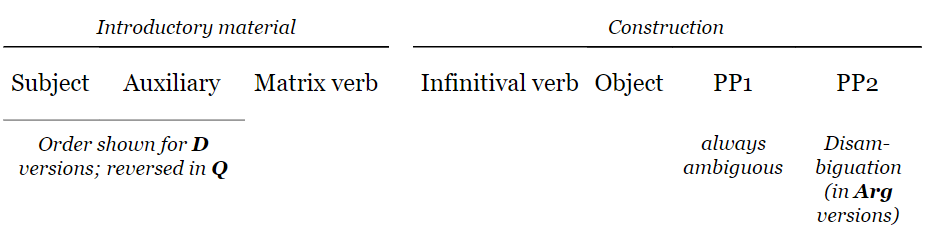
\includegraphics{item_diagram.png}
\end{enumerate}

All four versions of any given quadruple used the same introductory material, the only difference arising through the necessary inversion of auxiliary and matrix subject, as required by the Speech Act factor. Across quadruples, subjects alternated between \emph{she} and \emph{he}, with half using one and half using the other; the auxiliary was always \emph{had}. The matrix verb did not vary within a quadruple, but did vary between quadruples; for any given quadruple, the matrix verb was one of four verbs of mental state (\emph{decide}, \emph{intend}, \emph{plan}, or \emph{want}).

The verb within the construction did not vary within a quadruple, but a given quadruple could have one of four verbs: \emph{cram}, \emph{put}, \emph{set} or \emph{stick} The construction verb form was always infinitival. Each construction verb appeared in four different quadruples, and was paired once with each matrix verb, to create 16 unique pairings of matrix verb to construction verb. Thus, for matrix verb \emph{decide}, for example, \emph{decided to cram}, \emph{decided to put}, \emph{decided to set}, and \emph{decided to stick}; and for construction verb \emph{cram}, \emph{decided to cram}, \emph{intended to cram}, \emph{wanted to cram}, and \emph{planned to cram}.

The word order and content of the construction was the same across all versions of a quadruple, with the exception of the content of PP2 which varied across the PP2-Status factor: The Arg versions of a quadruple had a PP2 which was headed by \emph{into} or \emph{onto}, while the Mod versions had a PP2 which was headed by \emph{of} or \emph{from.}

PP1 was the same across versions of a given quadruple, e.g., \emph{cram the paperwork in the drawer\ldots{}} (see Table \ref{tab:sentences}'s illustrative example). That is, PP1 was identical (and temporarily ambiguous) in every version of a given quadruple, being interpretable as either the goal argument of the construction verb or as a modifier of the object NP. However, in Arg versions of a quadruple, the argument interpretation of PP1 cannot be sustained once PP2 is encountered. In those cases PP2 must fill the goal argument slot and PP1 must be a modifier. The working assumptions about parsing discussed earlier, i.e., that the parser will initially assume PP1 to be the goal argument due to the primary status of arguments, assumes that Arg versions of a quadruple require reanalysis. Between quadruples, the preposition that headed PP1 varied, but was always one which was compatible with it being a goal argument or a modifier of the object: \emph{in} (8), \emph{on} (7), and in one case, \emph{under.}

One benefit of using a complex verb cluster (auxiliary + matrix participle + infinitive) rather than a single verb\footnote{Note that the use of an auxiliary also eliminates length differences across D vs.~Q versions of a quadruple: if an auxiliary verb were not present, interrogative versions of a basic item would have an extra word, the result of so-called \emph{do}-support, that would not appear in the declaratives (e.g., \emph{he crammed} \ldots{} vs.~\emph{did he cram} \ldots{}?)} was that it isolated the differences across the versions of a quadruple triggered by the Speech Act factor to the left extremity of the introductory material of the sentence: only the position of the subject and the auxiliary were affected, meaning that the construction itself was completely untouched by this manipulation.

The purpose of including introductory matrix verbs was to reduce the oddity of the polar interrogative versions of each quadruple. It seems odd to ask, ``Did Mary put the jelly beans in the window onto a fancy dish?'' because, when it is clear that the speaker already knows so much about the situation, it becomes difficult to imagine a pragmatically plausible context where such a question would be asked. Such sentences might well be described as ``prosecutorial\footnote{Thank you to Dr.~Dianne Bradley for making this observation, and for the very clever ``prosecutorial'' descriptor.}.'' Arguably, this is somewhat mitigated by the addition of a verb like \emph{decided}: rather than asking about facts that we already seem to know, we are instead asking about an actor's mental state with regard to those facts. Even if we know the facts of the situation, we do not necessarily know, for instance, whether it was the result of a decision, some third party's action, or mere happenstance. Another adjustment made in order to make the polar interrogative versions of each quadruple more pragmatically acceptable limited the amount of detail in the experimental sentences, so that fewer adjectives and adverbs were included compared to the items employed in Peckenpaugh (2016), and subjects were always third person nominative pronouns (\emph{he} or \emph{she}).

Importantly, the construction verb was always one which demanded a goal argument. Where some of the verbs used in the items employed by Peckenpaugh (2016) only optionally took a goal, the current study used only verbs which require a goal argument. Verbs that optionally take a goal might result in a parse where PP1 is not immediately incorporated as the goal argument, which would mean that PP2 would not necessarily force reanalysis. Consider the contrasting sub-categorization of the verbs in (39) and (40):

\begin{enumerate}
\def\labelenumi{(\arabic{enumi})}
\setcounter{enumi}{38}
\item
  \textbf{Optional goal} (\emph{hide}) \linebreak
  The gangsters had hidden the shotguns in a U-Haul truck. \linebreak
  \(\checkmark\) The gangsters had hidden the shotguns. \linebreak
\item
  \textbf{Obligatory goal} (\emph{put}) \linebreak
  The gangsters had put the shotguns in a U-Haul truck. \linebreak
  \(*\) The gangsters had put the shotguns. \linebreak
\end{enumerate}

A verb like \emph{hide}, as in (39), can take a goal, but can also be used without one. A verb like \emph{put}, on the other hand, as in (40), really must have a goal. The use of verbs that require a goal argument in the current study maximized the likelihood of a robust garden path effect in the Arg versions, when PP2 triggered reanalysis. The four construction verbs used in this study were: \emph{cram}, \emph{put}, \emph{set} and \emph{stick}.

Another important consideration was ensuring that the Arg versions had a PP2 which definitively disambiguated the attachment site of PP1 such that reanalysis was forced. In (41), PP2 is implausible as a modifier of \emph{rocking horse}, but not strictly impossible, and the sentence is grammatical with PP2 modifying it. On the other hand, the use of \emph{onto} in (42) completely disallows the modifier interpretation of PP2 at the syntactic level: a PP headed by \emph{onto} cannot grammatically modify the preceding NP.

\begin{enumerate}
\def\labelenumi{(\arabic{enumi})}
\setcounter{enumi}{40}
\tightlist
\item
  She had decided to put the child {[}\textsubscript{PP1} on the rocking horse{]} {[}\textsubscript{PP2} on the see-saw{]}.
\item
  She had decided to put the child {[}\textsubscript{PP1} on the rocking horse{]} {[}\textsubscript{PP2} onto the see-saw{]}.
\end{enumerate}

Where Peckenpaugh (2016) relied on plausibility to force reanalysis, the current study uses syntactic disambiguation, such that the Arg versions always have a PP2 headed by \emph{into} or \emph{onto} which cannot head a PP2 that modifies the NP of PP1. This avoids any noise that might result from discrepancies between individuals' real world knowledge or beliefs. For the Mod items, the head preposition of PP2 was always either \emph{from} or \emph{of}, which are compatible with a parse where PP1 is the goal argument and PP2 is modifying the NP within PP1.

It is worth noting that some linguists (e.g., Den Dikken (2006)) believe \emph{of} is not a preposition in the same sense as \emph{from}, \emph{on}, or \emph{in}, etc., in that it appears to be serving a strictly grammatical or functional purpose, without real lexical content. Importantly, it is also only 2 characters, whereas \emph{into}, \emph{onto}, and \emph{from} (the other possible heads of PP2) are all 4 characters. This is revisited and its possible impact is explored in the results section (section \ref{pp2h}).

To sum up, the experimental items were designed to have limited detail, with either \emph{he} or \emph{she} as the matrix subject. A complex verb cluster, e.g., \emph{had decided to cram} was used to facilitate subject-auxiliary inversion without \emph{do}-support in the interrogatives and limit the difference between items, as well as provide a verb of mental state (\emph{decide}, \emph{intend}, \emph{plan}, or \emph{want}) to support more pragmatically plausible questions. PP1 was always interpretable as either the goal argument or a modifier of the object. PP2 differed across the PP2-Status factor, but not across the Speech Act factor. In the two Arg versions of a quadruple, it was headed by \emph{into} or \emph{onto} and was intended to force reanalysis, under the assumption that PP1 had been incorporated into the parse as an argument, since a PP headed by \emph{into} or \emph{onto} must be interpreted as the goal argument, the position that PP1 would have presumably been occupying in the ongoing parse. For the two Mod versions of a quadruple, PP2 was headed by \emph{from} or \emph{of} and therefore was not expected to require reanalysis, as \emph{from}- and \emph{of}-headed PPs can attach as modifiers of a preceding NP (in this case, the NP within PP1), allowing PP1 to stay in the goal argument slot.

\hypertarget{fillers}{%
\subsection{Fillers}\label{fillers}}

There were 32 filler items that ranged in complexity, e.g., some contained embedded finite or non-finite clauses, some contained reduced relative clauses or full relative clauses, and some were simple matrix clauses. Of these 32, 16 were designed to end in a sequence of two PPs, to mirror the experimental items (+PP), while the other half contained no final PPs (-PP). The +PP fillers were unrelated to the -PP fillers. All fillers were designed in two versions: declarative (D) and interrogative (Q). For the +PP fillers, PP1 was an argument in 5 of 16 cases, a modifier of the object in 6 cases, and a modifier of the verb phrase in 5 cases. The distribution of attachment sites for PP2 was the same, except there were 6 that modified the NP embedded in PP1 instead of 6 that modified the object. A full list of fillers is available in Appendix \ref{appFill}.

\begin{table}[!h]

\caption{\label{tab:fsentences}Illustrative filler items, constructed in two versions.}
\centering
\begin{tabular}{ll}
\toprule
Version & Sentence\\
\midrule
D +PP & He had forgotten to try the famous pastry in the restaurant of the fancy hotel.\\
Q +PP & Had he forgotten to try the famous pastry in the restaurant of the fancy hotel?\\
\hline
\addlinespace
D -PP & She had forgotten to report that the clerk was ignoring her request.\\
Q -PP & Had she forgotten to report that the clerk was ignoring her request?\\
\bottomrule
\end{tabular}
\end{table}

All filler items had the same sort of introductory material as the experimental items (\emph{he/she} + \emph{had} + past participle verb of mental state). The past participle was either one of the four mental state used for the experimental items (\emph{decide}, \emph{intend}, \emph{plan}, and \emph{want}), or one four additional verbs of mental state: \emph{forgot}, \emph{mean}, \emph{need}, or \emph{remember}, with each of the 8 past participles being used twice in the +PP fillers and twice in the -PP fillers, for a total of 4 times each. This means that a participant would see 6 instances each of \emph{decide}, \emph{intend}, \emph{plan}, and \emph{want}, but only 4 instances of the filler-only mental state verbs. Fillers used both mental state verbs from the experimental items as well as others was to prevent the experimental items as being identifiable by which mental state verb was used, and to avoid extreme amounts of repetition for any given lexical item.

\hypertarget{length}{%
\subsection{Length}\label{length}}

Length was tightly controlled across items. For experimental quadruples, all sentences were between 66 and 75 characters long, and between 13 and 15 words long. The length within a quadruple never varied across the D vs.~Q factor. Across the PP2-Status factor, given that the content of PP2 differed within a given quadruple, there was a maximum length difference of one character. Two quadruples varied in word length across PP2-Status by one word. Across all quadruples an equal number were longer (word- and character-wise) in the Arg condition as in the Mod condition. The experimental items ranged from 18 to 22 syllables.

Control over filler pair length was slightly less stringent. They ranged from 63 to 79 characters and 12 to 14 words. Length was never different within a filler pair, since only the Speech Act factor was implemented in the construction of fillers.

\hypertarget{participants-recruitment}{%
\section{Participants recruitment}\label{participants-recruitment}}

All participants in the were undergraduate students enrolled at Queens College in Psychology 101\footnote{IRB approval number: 2018-0072} who participated for course credit. Self-reported age ranged from 18 to 25 years. Participants were recruited a software system designed for university participant pools. Students saw a recruitment notice on the system website (see Appendix \ref{rec}), and were able to schedule their own appointment time within the hours offered.

The 35 participants recruited were self-identified native and primary speakers of American English. One participant was disqualified post-hoc after producing a Caribbean English pronunciation pattern; one further participant was excluded post-hoc due to an extremely disfluent reading cadence. A final participant was excluded due to a technical issue. All excluded participants were still awarded class credit for participating.

\hypertarget{location}{%
\section{Location}\label{location}}

All data were collected in a private room with only the experimenter and participant present. While every effort was undertaken to ensure a quiet environment, intrusive noise from passersby or neighboring rooms were sometimes unavoidable. This resulted in some unusable or partially unusable recordings (detailed in section \ref{irtDis} of the results chapter).

\hypertarget{equipment-and-software}{%
\section{Equipment and software}\label{equipment-and-software}}

The experiment was presented on a laptop running Windows 10 with stickers on the keyboard labeling relevant keys: the left shift key was labeled \emph{START}, right shift was labeled \emph{NEXT}, and the touch-pad was labeled \emph{DONE}.

The presentation of items and instruction\footnote{Instructions were also provided verbally and via printout, see Appendix \ref{instr}.} was done using the Open Sesame software (Mathôt, Schreij, \& Theeuwes, 2012) which provides a graphical user interface, scripting language, and interpretation of Python code. The system was capable of 10-20 millisecond accuracy, with the display's 60Hz refresh rate being the limiting factor. Key input had a latency of about 10ms.

Recording used a Blue Yeti USB microphone position near the participant's left hand and angled to point at the space in front of the participant's mouth. The angle was adjusted for each participant's height. Audio was recorded at 44.1kHz single-channel quality.

\hypertarget{versions-of-the-experiment}{%
\section{Versions of the experiment}\label{versions-of-the-experiment}}

The experiment was presented in 4 basic versions, with split-half ordering (where the first 24 of the items presented to one group was the second 24 presented to the other) for a total of 8 groups. Each version contained 7 practice items, 3 of which were overt practice and 4 of which were covert practice, as well as one version of each of the 16 experimental and 32 filler items. No version contained more than one version of a given experimental quadruple, or a given filler pair, and each version contained one member of every experimental quadruple and filler pair. Each participant saw the same number of each type of experimental quadruple: 4 D Arg, 4 Q Arg, 4 D Mod and 4 Q Mod. The experimental items were presented in pseudo-random order, interspersed with 1 to 3 fillers. Ignoring fillers, the same version of a different quadruple never occurred in sequence (e.g., after encountering a D Arg, the next experimental item was never another D Arg).

\hypertarget{procedure}{%
\section{Procedure}\label{procedure}}

Participants were given a verbal overview of the experimental procedure and then asked to read a one page review of the procedure (see Appendix \ref{instr}) before signing a consent form. Participants then sat at the computer and were again walked through instructions before the first practice item was presented.

Participants completed 3 practice items, then consulted with the experimenter before beginning the main portion of the study. The study also contained 4 covert practice items that were not included in any analyses, to allow participants to settle into the procedure before any results were recorded.

Participants used keyboard button presses to navigate the experimental presentation. Each such key-press terminated the current screen, and initiated display of the screen that was programmed to follow. The succession of 4 screens constituting the presentation of any item was participant-paced, as was the progress from item to item. Between items, the display defaulted to a fixation screen showing a line of ten pluses aligned with the left edge of the to-be-revealed sentence. This was designed to direct the participant's attention to the beginning of the sentence, and thus minimize unintended look-ahead (the issue of potential look-ahead is discussed at greater length in section \ref{look-ahead}). Items were uniformly presented without line breaks.

\begin{figure}
\centering
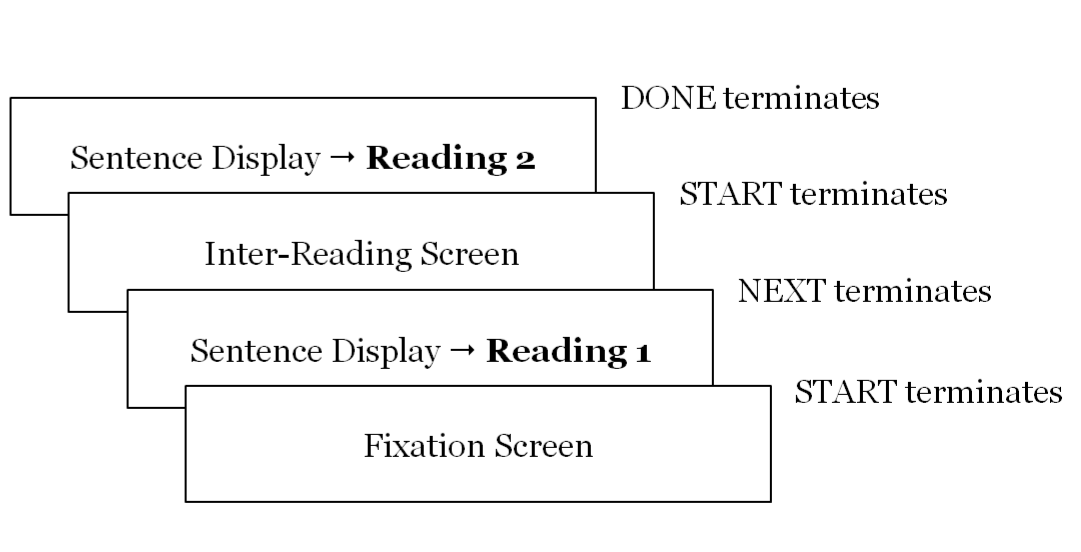
\includegraphics{procedure-diagram.png}
\caption{\label{fig:screens}Diagram of 4-screen sequence presented for each item, showing the key presses triggering movement between successive screens.}
\end{figure}

The first \emph{START} key-press that terminated the fixation screen and initiated the first display of a given item also began the first of the 2 recordings collected for each item. That recording continued through the presentation of the inter-item instruction slide and was terminated by the press of \emph{START} that terminated the inter-item instruction slide and initiated the second display of the item.

The second display of an item was displayed in black font on a pale blue background. All other screens were displayed in black font on a pale green background (i.e., fixation screen, first display of an item, and inter-item instruction screen, as well as the initial instructions).

The inter-item instruction slide which was displayed after the first display of an item was terminated contained the following text:

\begin{quotation}
Your first reading is complete.\\
Press START to begin the second reading.
\end{quotation}

The shifting of required key presses and the changing background color were intended to prevent accidental double-presses of any given button from having unintended side effects, and to help the participant track where in the protocol a given screen was located. It took some time for the participants to adapt to the procedure, but generally the necessary habits were acquired before the first item of the experiment proper was presented.

\hypertarget{look-ahead}{%
\subsection{On look-ahead}\label{look-ahead}}

An advantage that the Double Reading Procedure has is that it allows for certain assumptions to be made about Reading 2 that otherwise would be unclear: Reading 2 certainly represents a \emph{considered} reading of the sentence. Not only has the reader had ample time to examine the sentence, but has necessarily read it and heard it read in producing Reading 1. This means Reading 2 can plausibly be thought to represent a considered prosodic structure, at least more so than an entirely naive reading, and should not reflect any processing issues; a parse should have already been developed during Reading 1, or during subsequent study of the sentence prior to Reading 2.

The nature of Reading 1 is less clear. Because there is variability in the delay between the display of the sentence and the onset of phonation, it is possible that Reading 1 is not entirely delivered without preview. The properties of these Reading 1 delays are discussed at length in a later section, but for now it suffices to say that the very limited preview is possible during a delay that typically falls in the 0.2 to 2.7s range (median = 1s, SD = 0.4). As an example of common reading rates, Ashby, Yang, Evans, \& Rayner (2012) reported faster readers as averaging 328 words per minute (wpm), and slower readers 228wpm, in silent reading. That study found that reading time is slower for reading aloud, and that the availability of parafoveal information (i.e., the difference between 1 word and 3 word windows) is less impactful for that reading mode. Given that the experimental items range from 13 to 15 words, most of the R1 delays would not allow even a fast reader to read the entire sentence: the median 1s R1 delay would allow a fast reader time to read very few words; keep in mind that the window is even shorter, because in addition to just reading, the subject is also handling several other cognitive processes (e.g., visual processing, lexical access, issuing motor commands, etc.). The utterance of Reading 1 should, therefore, contain within it any behavioral reflex of whatever parsing difficult the reader has, for most recordings.

In order to clearly understand the results of this double reading study, it is important to understand the mechanics of reading. Specifically, we would want to know at what point during the reading of a temporarily ambiguous sentence the participant will become aware of the existence of a disambiguating PP2, since this is when it will be realized that the initial parse may well crash. The work of several decades on this subject is thoroughly summarized in Rayner, Pollatsek, Ashby, \& Clifton (2012). They describe reading as consisting of a series of fixations, when foveal vision takes in a small region of the visual field, and saccades, where the eyes move ahead ballistically (i.e., on a planned trajectory that cannot be interrupted). As a consequence of the ballistic property of saccadic movement and the additional finding that landing sites (fixations) are not random, we can infer that at least some look-ahead is available, i.e., a reader must know something about what is coming in order to plan a suitable landing site. The primary predictor of fixation point seems to be the character length of a word, meaning that the presence of characters and word boundary information (represented orthographically by spaces in languages like English) at least are necessary at the periphery of attention, i.e., within the perceptual span. Some details on the perceptual span, or the information that can be accessed by the eyes at any given time, is discussed in brief, with special attention to its relevance for the study at hand.

Rayner et al. (2012) discuss a number of studies that explore the size and properties of this span, the most fruitful of those studies being based on a gaze-contingent moving-window technique. In this technique, text is presented on a video monitor while the reader is also hooked up to eye-tracking equipment. A computer constantly samples the position of the reader's eyes and updates the display accordingly. Using this elaborate system, and the mutilation of text outside a window of clear text, a so-called moving window around the reader's point of fixation is created. By manipulating the size of this window, it was found that reading speed is maximized when about 15 characters to either side of the fixation site is available (it turns out this is actually asymmetric, and the window need only go as far as the start of currently fixated word in the direction of what has already been read, i.e., to the left for English readers).

In order to determine what information was available at the periphery of the perceptual span, the amount of information outside a window of clear text known to be smaller than the ideal (e.g., 21 characters, 10 to either side) was manipulated. When all characters and spaces were replaced with \emph{X}, essentially destroying all information outside the window, reading was slower than when character spaces were maintained, but all other information was obscured. Improvements in reading speed also occurred when characters were replaced with characters that had similar shape (i.e., the same pattern of ascenders and descenders) as the character they replaced, with and without spaces. Using these techniques and manipulating the size of the window, they were able to determine that it is only word boundary information that is available at the extreme edge of the perceptual span; character shape (ascenders and descenders) is available about 10 characters out from the fixation point, and character identity is available more or less only for the fixated word.

The relevant question for the study at hand is as follows: how much of the sentence will the reader have seen and processed when a given word is being spoken? A typical item is displayed in (43), with the words expected to be fixated underlined, numbered by presumed fixation sequence, and labeled. The number of characters (including spaces) intervening before the start of the disambiguating region (the left edge of PP2) is displayed below each label. These counts are calculated from the initial character of the fixated word to the initial character of the disambiguating region; the actual fixation site is likely to be closer to the center of the word, meaning the distance would be shortened by a few (1-4) characters, depending on the length of the fixated word.

\begin{enumerate}
\def\labelenumi{(\arabic{enumi})}
\setcounter{enumi}{42}
\item
\end{enumerate}

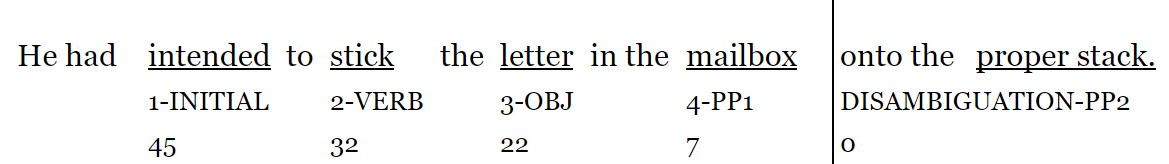
\includegraphics{distance-to-cr.png}

Table \ref{tab:dtcs} describes these distances across items all experimental items. Note that these values do not vary across condition, because counting starts after both the subject and auxiliary verb, and ends before PP2, and the only changes across versions are subject-auxiliary inversion and the content of PP2.

\begin{table}[!h]

\caption{\label{tab:dtcs}Distance in characters from fixation to disambiguation in experimental items.}
\centering
\begin{tabular}{rcccrcccrcccrcccrccc}
\toprule
  & 1-INITIAL & 2-VERB & 3-OBJ & 4-PP1\\
\midrule
Median & 46 & 34.5 & 25.5 & 7.5\\
Maximum & 50 & 38.0 & 27.0 & 9.0\\
Minimum & 45 & 32.0 & 21.0 & 5.0\\
\bottomrule
\end{tabular}
\end{table}

From the initial fixation point, the distance to disambiguation ranges from 45 to 50 characters, with a median of 46 characters. If we recall that word boundary information is available 15 to 18 characters to the right of fixation, we can be certain that the disambiguating region is far out of view until several fixations in.

When does the reader become aware of the existence of PP2? When fixated on the direct object head noun, the range of distance is 21 to 27 characters, with a median of 25.5: PP2's content is still outside of view, even in the case of the smallest distance, and adjusting it to be a few characters smaller to account for the fact that fixation is likely to occur closer to the center of a word rather than on its first character. At most, the presence of the first few characters of PP2's preposition may be available, but certainly not the character space after it. The distance from the PP1 fixation point (the head noun within that PP) ranges from 5 to 9 characters, with a median between 7 and 8 characters. Thus, we can say with some certainty that the reader of a sentence such as (43) will be aware that another phrase, one which starts with a 4-character word, remains to be incorporated into the parse sometime after processing of the direct object, and before processing of PP1.

There is yet another piece to consider: the so-called eye-voice span (EVS), and the fact that the readers in this study are reading aloud rather than silently. According to Laubrock \& Kliegl (2015), when reading aloud the voice is typically behind the eyes by some 10-20 characters (M = 16.2 characters, SD = 5.2 characters). Adjusting Table \ref{tab:dtcs} by subtracting 16 from each cell, we can approximate the position of the voice when the disambiguating region comes within the perceptual span. These values are shown in Table \ref{tab:evsdtcr}.

\begin{table}[!h]

\caption{\label{tab:evsdtcr}EVS-adjusted character distance to disambiguation in experimental items.}
\centering
\begin{tabular}{rcccrcccrcccrcccrccc}
\toprule
  & 1-INITIAL & 2-CONSTRUCTION VERB & 3-OBJ & 4-PP1\\
\midrule
Median & 30 & 18.5 & 9.5 & -8.5\\
Maximum & 34 & 22.0 & 11.0 & -7.0\\
Minimum & 29 & 16.0 & 5.0 & -11.0\\
\bottomrule
\end{tabular}
\end{table}

It is likely, then, an oral reader's voice would actually still be on the object when the eyes' fixation begins to provide information of some kind about the existence of PP2, and will still be pronouncing PP1 when the eyes are first fixated on PP2. This raises a question about any prosodic breaks produced after the object, because it is difficult to distinguish between an intentional prosodic break at that point, and one arising from the reader using a natural break for hesitation related to the garden path effect of discovering the disambiguating PP2.

\hypertarget{method-irt}{%
\section{Measurements of utterance timing}\label{method-irt}}

The elicitation protocol described above asked participants to read each sentence twice, once with no preview at all (Reading 1), and then again without any time pressure (Reading 2). Reading 1 (R1) delay is the elapsed time after a sentence is first displayed and when the participant begins speaking. Reading 2 (R2) delay is the same measure, but from the start of the second recording, which begins after the key press that terminates the inter-item instruction slide. Inter-reading time (IRT) is a measure of the time elapsing between when a participant stops speaking after R1 and when speaking resumes for R2. IRT encompasses but is not synonymous with R2 delay, because IRT also includes the elapsed time after the participant stops speaking and the end of the first recording. In this way, IRT is measured across both recordings.

The process for measuring makes use of Voice Activity Detection (VAD) software, which reports whether a given interval in a sound file contains speech-like noise. It's worth making clear that while VAD is employed, most of the measurements of interest are actually the inverse, i.e., the amount of time in a recording that does not contain speech-like noise. For each recording, the amount of time elapsed from the beginning of the recording to phonation onset and offset was found using VAD; then, R1 delay, R2 delay, utterance length and IRT were calculated as a function of each recording's length and the VAD-reported onset and offset of phonation.

The specific software used included a homemade Python script and Google's WebRTC VAD. The recordings were 44.1kHz WAV files down-sampled to 8kHz via SOX\footnote{Google's VAD API only accepts WAV files with sample rates that are a multiple of 8kHz. It ultimately down-samples all files to 8kHz, regardless of the input sampling rate.}. Google's VAD system used Gaussian Mixture Models to make probabilistic decisions as to whether a given audio frame was speech or noise (see Falk \& Chan (2006) for a complete description). Google's implementation takes one parameter called aggressiveness: a 4-tier setting for the level of confidence necessary to call a given interval speech. The implementation codes this setting on a 0-3 scale, where 0 is the most lenient (most likely to label a frame as speech) and 3 is the most stringent (most likely to label a frame as noise).

The recordings vary in the volume of the speaker's voice and the amount of background noise present. An algorithm was constructed to allow for the most stringent (highest VAD aggressiveness) measurement of the least modified data that gave plausible measurements. Specifically, each file was measured using the highest possible aggressiveness for the VAD algorithm and no modification of the recording. If the timings detected were not plausible, the timings were re-measured with the same rejection rate, but after the recording had undergone a 200Hz high-pass filter\footnote{The exact algorithm is available on \href{https://gist.github.com/moui72/4ebc4eb8f69eb9fdb1cab160ce299675}{github} (URL: \href{https://bit.ly/2uMrcrG}{bit.ly/2uMrcrG})} (HPF). If that still failed, a 400Hz HPF was used. After a further failure, the VAD aggressiveness was lowered, with each HPF value tried again (0, 200Hz, 400Hz); and that process was itself repeated until the lowest possible rejection rate was tried of the four possible settings. The majority of measurements were collected using the highest aggressiveness (85.4\%), with more than half requiring no HPF (59.6\%) and most of the request requiring a 200Hz HPF (40.1\%).

A plausible set of measurements was required to meet the following criteria:

A. \emph{Utterance length:} An utterance length between 2s and 10s, where utterance timing is the longest contiguous span in the recording that VAD reports as phonation, with breaks in phonation of less than 1s not breaking contiguity, as Goldman-Eisler (1961) found that a large majority (82.5 to 87\%) of pauses in fluent speech are less than 1s. Stimuli range from 18-22 syllables in length. If we assume a speech rate of 3 to 7 syllables per second (Jacewicz, Fox, \& Wei, 2010) we would expect utterances between 2.5s and 7.3s. Conservative thresholds higher and lower than the expected were used, especially on the higher end, to allow for any difficulties processing or fluency that might have lead to longer reading times.

B. \emph{Minimum leading silence:} A leading silence (``delay'') of more than 120ms. Even a very fast human reaction time should not permit a delay shorter than 120ms, so a shorter delay likely means an inaccurate set of measurements has been reported.

C. \emph{Maximum edge silence:} A maximum trailing and leading silence length of less than 95\% of the file's length was also used, in order to filter out recordings that do not represent a valid trial. Very long silences less than this very conservative threshold that impact the IRT are dealt with in the data clean-up rather than via phonation detection, as described in the results section of this paper (section \ref{irtDis}).

With 32 participants reading 48 items (experimental and filler) twice each, there are an expected number of 3072 recordings; due to technical issues at the time of data collection, 71 recordings are missing. Of the 3001 recordings subjected to this treatment, 2976 resulted in plausible timings{[}\^{}handset{]}. A review of those that did not result in plausible timings found 9 recordings that were too noisy for computer analysis, but still usable, and those timings were recorded by hand.

To verify the accuracy of the computer measurement, timings were collected by hand for 240 recording. There was a significant positive correlation between hand-measured and computer-measured timings (r(118)=0.87, p \textless{} 0.001), with a median difference of 0.4s\footnote{Hand measurement was done to the nearest half second, so a fair amount of error is to be expected.} (SD = 1.5).

\hypertarget{sita}{%
\section{Prosodic judgments}\label{sita}}

A trained linguist informant naive to the research being conducted listened to recordings and reported the presence or absence of breaks in certain regions\footnote{She also reported on a break after the construction verb, but that break was so rare that it is ignored throughout this report.} of the sentence, as well as several other judgments. She was instructed to familiarize herself with a speaker's speech patterns before rating any recordings by listening to 6 filler item recordings from that speaker. She was given a diagram of the sentences as in (44), as well as full plain-text lists of all items.

\begin{enumerate}
\def\labelenumi{(\arabic{enumi})}
\setcounter{enumi}{43}
\tightlist
\item
  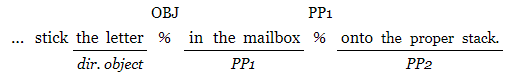
\includegraphics{breakpos.png}
\end{enumerate}

She was asked to report on whether or not she heard a prosodic boundary directly following the region labeled \textbf{OBJ}, and directly after the following labeled \textbf{PP1}. The following definition of prosodic break was provided:

\begin{quote}
Please work with the assumption that ``prosodic boundary'' in what follows is any subset of the following features, clustered in such a way as to trigger your intuition that a new prosodic element (of any size) is beginning: pitch change, volume change, segmental lengthening, or pause.
\end{quote}

The judgments requested also included whether or not the speaker struggled, where that struggle began, whether or not the speaker used question intonation, and which break(s) were stronger or more prominent than which other break(s).

Detailed instructions on the order in which items should be listened to, both within speaker and across speakers, were also provided. The result was that she never listened to both readings of a sentence in sequence; she never listened to 2 Reading 1 versions of different sentences in sequence; and she never listened to the sentences in the same order for a given participant as she did for the previous one.

Details on the instructions given and the judgments collected can be found in Appendix \ref{RA}.

This strict procedure was implemented to hinder the informant from recognizing any patterns in the data, e.g., a systematic difference between Readings 1 and 2. It also mitigated any ordering effects that might occur in the data or as a result of the informant's own process. The familiarization process via filler items allowed the informant to judge the existence of breaks relative to the typical cadence and fluency of a given speaker, prior to exposure to any of the experimental items for that speaker.

\hypertarget{rel}{%
\subsection{Reliability}\label{rel}}

A second trained linguist repeated the task over 120 recordings selected from 8 participants (two from each group, one per ordering). Even number experimental items were used from 4 participants, and odd numbered from the other 4. There were 8 recordings missing from the 128 selected, so the reliability task resulted in judgments over 120 recordings. The first informant also blindly re-rated those 120, with the recording name obscured and instructions not to revisit her original ratings. Reliability scores (percent of recordings agreed upon) are reported in Table \ref{tab:validity}.

\begin{table}[!h]

\caption{\label{tab:validity}Inter and intra-rater agreement.}
\centering
\begin{tabular}{>{\bfseries}cccc}
\toprule
  & OBJ & PP1 & Break strength\\
\midrule
 & 65.0\% & 78.3\% & 54.2\%\\

 & K = 0.17** & K = 0.09 . & K = 0.25***\\

\multirow{-3}{*}{\centering\arraybackslash Inter-rater} & (z = 2.61) & (z = 1.86) & (z = 3.99)\\
\cmidrule{1-4}
 & 77.5\% & 85.0\% & 72.5\%\\

 & K = 0.52*** & K = 0.52*** & K = 0.44***\\

\multirow{-3}{*}{\centering\arraybackslash Intra-rater} & (z = 5.73) & (z = 5.82) & (z = 5.70)\\
\bottomrule
\multicolumn{4}{l}{\textit{Note: }}\\
\multicolumn{4}{l}{*** p < 0.001; ** p < 0.01; * p < 0.05, . p < 0.1}\\
\end{tabular}
\end{table}

The lower intra-rater agreement for relative break strength was likely impacted by the method of reporting: because the informant was actually asked to provide judgments over three break locations (the third, V, is omitted throughout this report because it was extremely rare, occurring in just over 8\% of recordings). As such, disagreement on that break and the fact that break strength is actually a compilation of two judgments (weakest and strongest break) amplified the noise to some extent.

\hypertarget{res}{%
\chapter{Results and discussion}\label{res}}

This section reports various descriptions and analyses of the recordings obtained, and the relevance of those findings to the research questions motivating this study. The reported results include the effect of Speech Act (declarative/D vs.~interrogative/Q) and PP2 Status (argument/Arg vs.~modifier/Mod) on the location of prosodic breaks, as well as on time spent reflecting upon a sentence between readings, which I call inter-reading time (IRT). In order to evaluate the extent to which participants adhered to the protocol as intended, i.e., began to read immediately for Reading 1 as opposed to producing a considered reading in Reading 2, the delay for which a sentence is displayed before a participant begins to read it is compared for Reading 1 (R1 delay) vs.~Reading 2 (R2 delay). The prosodic patterns for participants with especially fast and especially slow R1 delays are presented as a way of investigating the extent to which individual differences might impact those patterns, and as a further exploration of the success of the protocol instructions in producing the intended behavior. A finding on the apparent processing cost of interrogative context when compared to declarative context among the filler sentences is also reported.

\hypertarget{data-for-analysis}{%
\section{Data for analysis}\label{data-for-analysis}}

Data for 32 total participants were analyzed. Given 4 versions of the experiment and 2 possible orderings there would ideally be 4 participants per version-order combination. Ultimately, 3 participants had to be excluded for different reasons, resulting in the distribution is as shown in Table \ref{tab:vtab}\footnote{The two 5-count cells include 2 additional participants whose data were collected in pursuit of another full set (i.e., towards an expansion to 40 participants) that was not completed due to a lack of participant sign-ups.}. Participants were removed for the following reasons: one for use of a non-standard dialect, one for extremely disfluent oral reading, and one who was missing more than half of the expected recordings because of a system crash during the procedure.

\begin{table}[!h]

\caption{\label{tab:vtab}Number of participants per version-order combination.}
\centering
\begin{tabular}{lccc}
\toprule
\multicolumn{1}{c}{ } & \multicolumn{2}{c}{Order} & \multicolumn{1}{c}{ } \\
\cmidrule(l{3pt}r{3pt}){2-3}
  & 1 & 2 & Sum\\
\midrule
Version 1 & 5 & 4 & 9\\
Version 2 & 4 & 4 & 8\\
Version 3 & 4 & 4 & 8\\
Version 4 & 2 & 5 & 7\\
Sum & 15 & 17 & 32\\
\bottomrule
\end{tabular}
\end{table}

Some of the expected 3072 recordings (32 participants x 48 items (16 experimental and 32 filler) x 2 readings) were not used due to intrusive noise during the recording session. Additionally, data were also excluded from analysis if any (Reading 1/Reading 2 pair) was missing; there were 9 such incomplete pairs excluded. Without analyzable data from both members of a pair, it is difficult to determine the extent to which the elicitation protocol was executed as intended (i.e., the extent of preview for Reading 1 vs.~Reading 2).

For experimental items, 978 recordings were subjected to prosodic analysis, constituting 95.6\% of the utterances elicited. Because IRT data considered utterances in pairs (Reading 1/Reading 2) rather than separately, the database for response timing took in 489 data points.

\begin{table}[!h]

\caption{\label{tab:rvtab}Number of recordings analyzed, as a function of Speech Act and PP2 Status.}
\centering
\begin{tabular}{ccc}
\toprule
  & D & Q\\
\midrule
Arg & 244 & 240\\
Mod & 246 & 248\\
\bottomrule
\end{tabular}
\end{table}

\hypertarget{results-prosody}{%
\section{Prosodic break patterns}\label{results-prosody}}

The section will report the prosodic phrasings found in the recordings collected, and the extent to which those patterns are or are not influenced by the design parameters of the study (Speech Act and PP2 Status), as well as which reading (Reading 1 or Reading 2) the recording represents. This reported first descriptively (i.e., in terms of frequency), and then using regression models to calculate the statistical significance of whatever effects are found. Finally, a summary of findings and their implications for the hypothesis motivating this study is provided.

In what follows, the distribution of OBJ breaks and PP1 breaks are reported as a function of the four sentence types created by the materials design (D/Q x Arg/Mod), for each of Reading 1 and Reading 2. Then, the patterns of breaks over the two positions are considered, before moving to statistical analysis. Note that while breaks after the construction verb were reported, these breaks were exceptionally rare and occurred in only 8\% of recordings, so they have been set aside. The break locations are indicated with a \% symbol in (45).

\begin{enumerate}
\def\labelenumi{(\arabic{enumi})}
\setcounter{enumi}{44}
\tightlist
\item
  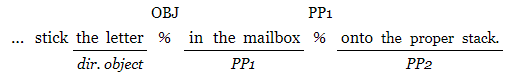
\includegraphics{breakpos.png}
\end{enumerate}

As noted in section \ref{sita}, the results reported are based on the subjective judgments of a trained linguist who was naive to the purposes and hypotheses underlying the research.

\hypertarget{individual-break-patterns}{%
\subsection{Individual break patterns}\label{individual-break-patterns}}

\begin{table}[!h]

\caption{\label{tab:obj}Percent occurrence of OBJ break (frequency of occurrence in parenthesis) as a function of sentence type and Reading.}
\centering
\begin{tabular}{ccccc}
\toprule
\multicolumn{1}{c}{ } & \multicolumn{2}{c}{Reading 1} & \multicolumn{2}{c}{Reading 2} \\
\cmidrule(l{3pt}r{3pt}){2-3} \cmidrule(l{3pt}r{3pt}){4-5}
 & D & Q & D & Q\\
\midrule
Arg & 57.4\% (70) & 56.7\% (68) & 73.0\% (89) & 74.2\% (89)\\
Mod & 77.2\% (95) & 76.6\% (95) & 84.6\% (104) & 72.6\% (90)\\
\bottomrule
\end{tabular}
\end{table}

The presence of the OBJ break was sensitive to both Speech Act and reading, with Reading 2 showing a different distribution across the D vs.~Q distinction than the Reading 1 recordings.

\begin{table}[!h]

\caption{\label{tab:pp1}Percent occurrence of PP1 break (frequency of occurrence in parenthesis) as a function of sentence type and Reading.}
\centering
\begin{tabular}{ccccc}
\toprule
\multicolumn{1}{c}{ } & \multicolumn{2}{c}{Reading 1} & \multicolumn{2}{c}{Reading 2} \\
\cmidrule(l{3pt}r{3pt}){2-3} \cmidrule(l{3pt}r{3pt}){4-5}
 & D & Q & D & Q\\
\midrule
Arg & 121 (99.2\%) & 119 (99.2\%) & 121 (99.2\%) & 117 (97.5\%)\\
Mod & 84 (68.3\%) & 85 (68.5\%) & 84 (68.3\%) & 83 (66.9\%)\\
\bottomrule
\end{tabular}
\end{table}

The PP1 break was almost always present for cases where PP2 was an argument; and it was present substantially less often, but still there a majority of the time, for cases where PP2 could be interpreted as a modifier. Speech act and reading did not appear to impact the overall distribution of the PP1 break.

\hypertarget{bbr}{%
\subsection{Combined break patterns}\label{bbr}}

When looking at both breaks together, a sentence could have one of four patterns: both the OBJ and PP1 break present; only OBJ present; only PP1 present; or neither break present. There were only 5 cases where neither was present, and those were omitted in the tables of prosodic patterns.

\begin{table}[!h]

\caption{\label{tab:bothbreaks}Percent occurrence of both breaks as a function of sentence type and Reading.}
\centering
\begin{tabular}{>{\bfseries}lcccccccc}
\toprule
\multicolumn{1}{c}{ } & \multicolumn{4}{c}{Reading 1} & \multicolumn{4}{c}{Reading 2} \\
\cmidrule(l{3pt}r{3pt}){2-5} \cmidrule(l{3pt}r{3pt}){6-9}
\multicolumn{1}{c}{ } & \multicolumn{2}{c}{Mod} & \multicolumn{2}{c}{Arg} & \multicolumn{2}{c}{Mod} & \multicolumn{2}{c}{Arg} \\
\cmidrule(l{3pt}r{3pt}){2-3} \cmidrule(l{3pt}r{3pt}){4-5} \cmidrule(l{3pt}r{3pt}){6-7} \cmidrule(l{3pt}r{3pt}){8-9}
  & D & Q & D & Q & D & Q & D & Q\\
\midrule
OBJ only & 31.1\% & 31.4\% & 0.8\% & 2.5\% & 31.7\% & 30.9\% & 0.8\% & 0.8\%\\
Both & 54.1\% & 43.0\% & 72.1\% & 71.7\% & 45.5\% & 46.3\% & 56.6\% & 55.8\%\\
PP1 only & 14.8\% & 25.6\% & 27.0\% & 25.8\% & 22.8\% & 22.8\% & 42.6\% & 43.3\%\\
\bottomrule
\end{tabular}
\end{table}

Table \ref{tab:bothbreaks} shows that for Arg sentences, there are very few instances with the OBJ-only pattern (0.8\% in declaratives, 2.5\% in interrogatives); whereas that pattern is fairly frequent for Mod sentences (31.1\% in declaratives, 31.4\% in interrogatives). The pattern with both breaks is somewhat more common for Arg sentences (72.1\% in declaratives, 71.7\% in interrogatives) than Mod (54.1\% in declaratives, 43.0\% in interrogatives). The PP1-only pattern occurs at about the same rate in Arg interrogatives (25.8\%) as in Mod interrogatives (25.6\%) and Arg declaratives (27\%), but is noticeably less common for Mod declaratives (14.8\%). These proportions are visually represented in figure \ref{fig:bothbreaks2}.

\begin{figure}
\centering
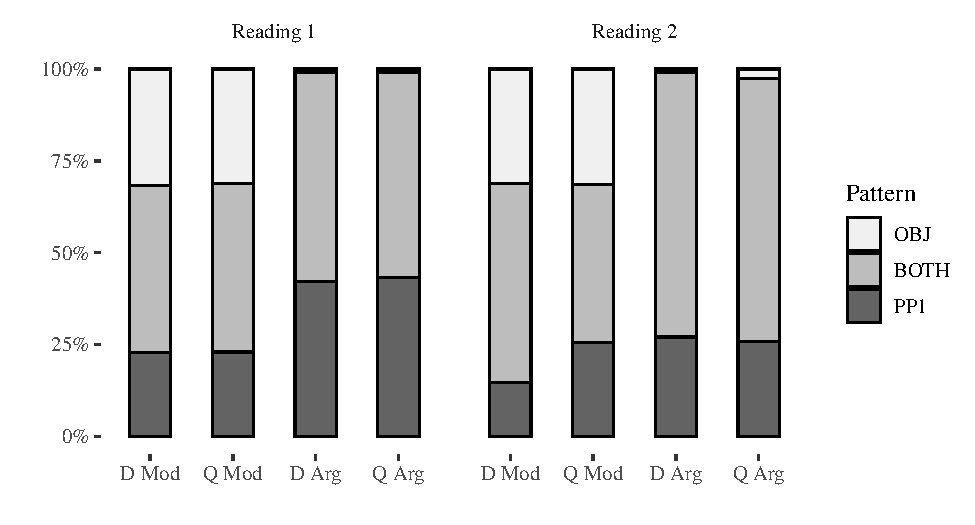
\includegraphics{4-results_files/figure-latex/bothbreaks2-1.pdf}
\caption{\label{fig:bothbreaks2}Break pattern as a function of sentence type and Reading.}
\end{figure}

\hypertarget{break-dominance}{%
\subsection{Break Dominance}\label{break-dominance}}

The relative strength of the PP1 and OBJ breaks was also collected. Figure \ref{fig:bdom} incorporates this information, where ``PP1 dominance'' means that the PP1 break was reported to be stronger than the OBJ break; ``OBJ'' dominance means the opposite; and ``Equal strength'' means that neither break was reported to be stronger than the other (the 5 instances with no breaks were again omitted).

When looking at the combined break patterns, one can think of there being three bins: the PP1 bin, the OBJ bin, and a neutral bin between them. In Section \ref{bbr}, the neutral bin containing instances of both breaks occurring is robust. This break dominance analysis distributes most of those cases that have both breaks into either the OBJ or PP1 bin, depending on which break is more prominent. When the breaks are of equal strength, they remain in the middle bin, but there are much fewer such cases when looking at dominance instead of simple occurrence.

\begin{figure}
\centering
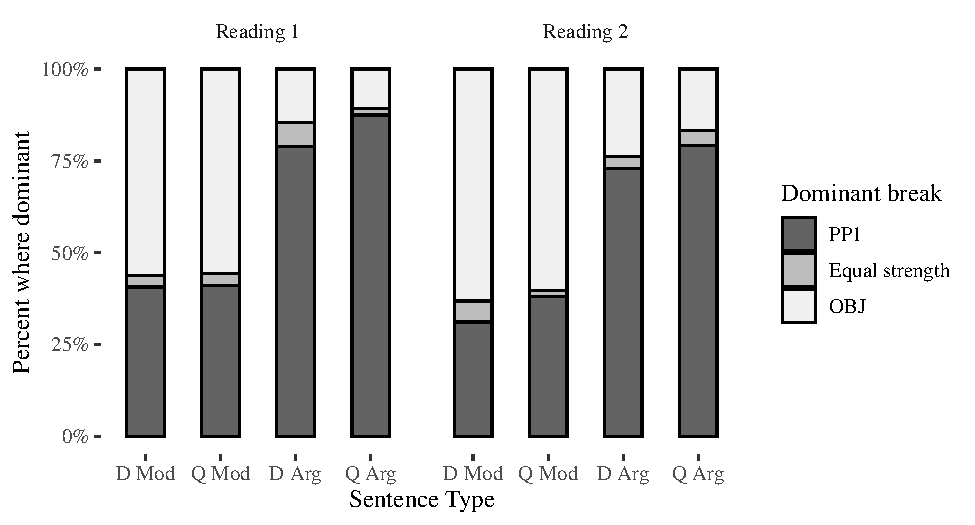
\includegraphics{4-results_files/figure-latex/bdom-1.pdf}
\caption{\label{fig:bdom}Percent break dominance occurence as a function of sentence type and Reading.}
\end{figure}

Figure \ref{fig:bdom} clearly shows a robust effect of PP2 Status on break dominance, and little to no impact of Reading or Speech Act.

\hypertarget{regression-models-of-prosodic-break-patterns}{%
\subsection{Regression models of prosodic break patterns}\label{regression-models-of-prosodic-break-patterns}}

A number of mixed effects logistic regression models support the general observations above. Models predicting PP1 break, OBJ break, PP1 break dominance and OBJ break dominance are reported. All models include crossed random effect intercepts (participant and item), but due to convergence errors, no random slopes for any predictors are included.

The intercept always represents the Mod sentence type, which is not expected to present any particular difficulty to the reader, since the Mod PP2 Status is compatible with what is assumed to be the running parse when it is encountered (i.e., PP1 has been interpreted as the goal argument of the verb, and PP2 does not disrupt that interpretation). For those models where Speech Act is included in the model, the intercept represents the declarative sentence type. In this way, the more complex sentence types are compared to the simplest available in the model. If Reading is included in a model, the intercept represents Reading 1.

For each analysis, a reduced model and the full model (i.e., the model containing all predictors of interest) is reported. In each case, the reported reduced model is the one with the lowest reported Akaike Information Criterion\footnote{AIC is a representation of the amount of information lost by using a regression model to estimate data points. It is a measure that balances both the goodness of fit of a model and the simplicity of a model, guarding against over fitting and under fitting the data involved.} (AIC) from the set of models that include any subset of the following predictors: Speech Act, PP2 Status, Reading, and the interactions between Speech Act, PP2 Status and Reading. This method of model selection is consistent with the proposal of Wax \& Kailath (1985).

Model comparisons did not always find significant differences between the more complex models, but in each case, the selected model was compared to a minimal model where where fixed effect variables were removed, leaving only an intercept, and all reported models represent improvement over the minimal model to a statistically significant degree. That comparison is reported for each model. All regression models were run using the lme4 R package (Bates, Maechler, Bolker, \& Walker (2019)), with p-values calculated via the lmerTest R package (Kuznetsova, Bruun Brockhoff, \& Haubo Bojesen Christensen (2019)).

\hypertarget{break-occurrence}{%
\subsubsection{Break occurrence}\label{break-occurrence}}

In the full model predicting OBJ break occurrence, shown in Table \ref{tab:fullobjmod}, only the estimate for D Mod Reading 1 (the intercept) and the effect of PP2 Status show statistical significance.

\begin{table}[!h]

\caption{\label{tab:fullobjmod}Mixed effects logistic regression model predicting OBJ break occurrence (FULL).}
\centering
\begin{tabular}{rcccrcccrcccrccc}
\toprule
\multicolumn{1}{c}{Outcome: OBJ break (FULL)} & \multicolumn{1}{c}{Estimate} & \multicolumn{1}{c}{Std. Error} & \multicolumn{1}{c}{p}\\
\midrule
D Mod, Reading 1 (Intercept) & 0.70 & 0.09 & < 0.001\\
Q & 0.11 & 0.11 & 0.34\\
Arg & -0.28 & 0.11 & < 0.05\\
Reading 2 & 0.07 & 0.05 & 0.15\\
Q:Arg & -0.14 & 0.16 & 0.39\\
\addlinespace
Q:Reading2 & -0.11 & 0.07 & 0.12\\
Arg:Reading2 & 0.08 & 0.07 & 0.27\\
Q:Arg:Reading2 & 0.13 & 0.10 & 0.19\\
\bottomrule
\end{tabular}
\end{table}

Table \ref{tab:objMod} shows a reduced model, predicting the occurrence of an OBJ break with estimates for the coefficients of the fixed effects of Reading 2, PP2 and the interaction between Reading and PP2 Status. The removal of other predictors allowed the Reading x PP2 Status to become a significant predictor. A comparison between the reported model and a minimal one found that the reported model was better with a high level of confidence (AIC\textsubscript{MIN}=1068.0, AIC\textsubscript{BEST}=1031.6, \(\chi^2\)(2)=30.5, p \textless{} 0.001).

\begin{table}[!h]

\caption{\label{tab:objMod}Mixed effects logistic regression model predicting OBJ break occurrence (REDUCED).}
\centering
\begin{tabular}{rcccrcccrcccrccc}
\toprule
\multicolumn{1}{c}{Outcome: OBJ break (REDUCED)} & \multicolumn{1}{c}{Estimate} & \multicolumn{1}{c}{Std. Error} & \multicolumn{1}{c}{p}\\
\midrule
D Mod, Reading 1 (Intercept) & 1.39 & 0.45 & < 0.01\\
Reading 2 & 0.11 & 0.23 & 0.62\\
Arg & -1.98 & 0.50 & < 0.001\\
Reading 2 x Arg & 0.81 & 0.32 & < 0.05\\
\bottomrule
\end{tabular}
\end{table}

The log odds\footnote{Log odds is, in this case, the natural log of the odds ratio, so the log odds of A is log\textsubscript{e}(P(A)/P(¬A)). A log odds of 1.39 translates to an odds ratio of 4.01:1 (1.39\textsuperscript{e}=4.01) and a probability of 80\% (4.01/(1+4.01)=0.80).} of an OBJ break for Mod Reading 1 is 1.39 (std. error = 0.45, p \textless{} 0.01). The log odds of that break increased in Reading 2 but the increase was not statistically significant. PP2 arguments reduced the log odds of an OBJ break compared to PP2 modifiers by a robust amount, but less so in Reading 2 than in Reading 1.

The OBJ break is expected to occur more often in Mod cases, because that break marks the argument attachment (and therefore a change in branching direction) of PP1.

The full model for predicting PP1 also showed significance only for the intercept and the effect of PP2 Status.

\begin{table}[!h]

\caption{\label{tab:fullpp1Mod}Mixed effects logistic regression model predicting PP1 break occurrence (FULL).}
\centering
\begin{tabular}{rrrlrrrlrrrlrrrl}
\toprule
\multicolumn{1}{c}{Outcome: PP1 break (FULL)} & \multicolumn{1}{c}{Estimate} & \multicolumn{1}{c}{Std. Error} & \multicolumn{1}{c}{p}\\
\midrule
D Mod, Reading 1 (Intercept) & 0.68 & 0.07 & < 0.001\\
Q & 0.01 & 0.09 & 0.89\\
Arg & 0.31 & 0.09 & < 0.001\\
Reading 2 & 0.00 & 0.04 & 1.00\\
Q:Arg & 0.00 & 0.13 & 0.97\\
\addlinespace
Q:Reading2 & -0.01 & 0.06 & 0.82\\
Arg:Reading2 & 0.00 & 0.06 & 1.00\\
Q:Arg:Reading2 & 0.00 & 0.08 & 0.97\\
\bottomrule
\end{tabular}
\end{table}

The best model for predicting the occurrence for the PP1 break was one where only PP2 Status was included as a predictor. The chosen model was again significantly better than the minimal model (AIC\textsubscript{MIN}=855.6, AIC\textsubscript{BEST}=629.6, \(\chi^2\)(1)=228.0, p \textless{} 0.001).

\begin{table}[!h]

\caption{\label{tab:pp1Mod}Mixed effects logistic regression model predicting PP1 break occurrence (REDUCED).}
\centering
\begin{tabular}{rcccrcccrcccrccc}
\toprule
\multicolumn{1}{c}{Outcome: PP1 break (REDUCED)} & \multicolumn{1}{c}{Estimate} & \multicolumn{1}{c}{Std. Error} & \multicolumn{1}{c}{p}\\
\midrule
Mod (Intercept) & 0.96 & 0.30 & < 0.01\\
Arg & 4.12 & 0.44 & < 0.001\\
\bottomrule
\end{tabular}
\end{table}

Sentences with argument PP2s had greatly increased log odds of a PP1 break compared to ones with modifier PP2s. This is again expected, because the PP1 break is indicating the change in branching direction for argument attachment of PP2. That Speech Act is not a relevant predictor is evidence against a prosodic explanation of the motivating intuition for this study; we would expect both a main effect of Speech Act and definitely an interaction between Speech Act and PP2 Status, if the prosody were more or less different across the PP2 Status factor for interrogatives than for declaratives.

\hypertarget{break-dominance-1}{%
\subsubsection{Break dominance}\label{break-dominance-1}}

Models were also run for predicting break dominance. The full model predicting OBJ break dominance is shown in Table \ref{tab:fodom}.

\begin{table}[!h]

\caption{\label{tab:fodom}Mixed effects logistic regression model predicting OBJ break dominance (FULL).}
\centering
\begin{tabular}{rcccrcccrcccrccc}
\toprule
\multicolumn{1}{c}{Outcome: OBJ dominance (FULL)} & \multicolumn{1}{c}{Estimate} & \multicolumn{1}{c}{Std. Error} & \multicolumn{1}{c}{p}\\
\midrule
D Mod, Reading 1 (Intercept) & 0.50 & 0.09 & < 0.001\\
Q & 0.03 & 0.12 & 0.82\\
Arg & -0.45 & 0.12 & < 0.001\\
Reading 2 & 0.07 & 0.05 & 0.22\\
Q:Arg & -0.03 & 0.17 & 0.86\\
\addlinespace
Q:Reading2 & -0.03 & 0.07 & 0.68\\
Arg:Reading2 & 0.03 & 0.07 & 0.71\\
Q:Arg:Reading2 & 0.00 & 0.11 & 0.97\\
\bottomrule
\end{tabular}
\end{table}

Table \ref{tab:odom} reports the best model for predicting OBJ break dominance. The best model was one with fixed effects for reading and PP2 Status. There was no statistically significant effect of Speech Act on OBJ break dominance.

\begin{table}[!h]

\caption{\label{tab:odom}Mixed effects logistic regression model predicting OBJ break dominance (REDUCED).}
\centering
\begin{tabular}{rcccrcccrcccrccc}
\toprule
\multicolumn{1}{c}{Outcome: OBJ dominance (REDUCED)} & \multicolumn{1}{c}{Estimate} & \multicolumn{1}{c}{Std. Error} & \multicolumn{1}{c}{p}\\
\midrule
Mod, Reading 1 (Intercept) & -0.16 & 0.32 & 0.62\\
Reading 2 & 0.40 & 0.16 & < 0.05\\
Arg & -2.32 & 0.18 & < 0.001\\
\bottomrule
\end{tabular}
\end{table}

PP1 break dominance and OBJ break dominance are not entirely complementary, because it is possible for both breaks to have equal prominence. As such, models predicting PP1 were also explored.

The full model predicting PP1 break dominance failed to converge, so only the reduced model is reported.

Table \ref{tab:pdom} reports the best model for predicting PP1 break dominance. Unlike the model for predicting OBJ break dominance, the best model for predicting PP1 break dominance includes Speech Act as a predictor. The best model is one with fixed effects for reading, Speech Act, and PP2 Status.

\begin{table}[!h]

\caption{\label{tab:pdom}Mixed effects logistic regression model predicting PP1 break dominance (REDUCED).}
\centering
\begin{tabular}{rcccrcccrcccrccc}
\toprule
\multicolumn{1}{c}{Outcome: PP1 dominance (REDUCED)} & \multicolumn{1}{c}{Estimate} & \multicolumn{1}{c}{Std. Error} & \multicolumn{1}{c}{p}\\
\midrule
D Mod, Reading 1 (Intercept) & -0.19 & 0.33 & 0.57\\
Reading 2 & -0.38 & 0.15 & < 0.05\\
Q & 0.31 & 0.15 & < 0.05\\
Arg & 2.20 & 0.17 & < 0.001\\
\bottomrule
\end{tabular}
\end{table}

This model was better than a minimal model (AIC\textsubscript{MIN}=1290.4, AIC\textsubscript{BEST}=1078.8, \(\chi^2\)(3)=217.59, p \textless{} 0.001). PP1 break dominance was much more likely for sentence with argument PP2s than sentences with modifier PP2s, with interrogatives having slightly increased log odds of PP1 break dominance. Log odds of PP1 break dominance were slightly less in Reading 2 than Reading 1. There were no significant interaction terms.

Because reading was a significant predictor for 3 of the 4 models reported, and there are theoretical reasons to believe that Reading 2 is more representative of the natural or intended prosody of the reader, models were also run predicting PP1 dominance and OBJ dominance for Reading 2 data only. In both cases, the best model had the same structure: fixed effects of Speech Act and PP2 Status, with no interaction term.

\begin{table}[!h]

\caption{\label{tab:r2dom}Mixed effects logistic regression models predicting break dominance in Reading 2 (REDUCED).}
\centering
\begin{tabular}{rcccrcccrcccrcccrcccrcccrccc}
\toprule
\multicolumn{1}{c}{ } & \multicolumn{3}{c}{Outcome: OBJ Dominance} & \multicolumn{3}{c}{Outcome: PP1 Dominance} \\
\cmidrule(l{3pt}r{3pt}){2-4} \cmidrule(l{3pt}r{3pt}){5-7}
\multicolumn{1}{c}{(Reading 2 only)} & \multicolumn{1}{c}{Estimate} & \multicolumn{1}{c}{Std. Err} & \multicolumn{1}{c}{p} & \multicolumn{1}{c}{Estimate} & \multicolumn{1}{c}{Std. Err} & \multicolumn{1}{c}{p}\\
\midrule
D Mod (Intercept) & 0.66 & 0.24 & < 0.01 & -0.97 & 0.27 & < 0.001\\
Q & -0.30 & 0.22 & 0.16 & 0.35 & 0.22 & 0.1\\
Arg & -2.07 & 0.24 & < 0.001 & 2.15 & 0.24 & < 0.001\\
\bottomrule
\end{tabular}
\end{table}

For both OBJ dominance and PP2 dominance, the main effect of Speech Act is non-significant, but its inclusion marginally improves the fit of each model. Even when limited to only Reading 2 data, Speech Act does not interact with PP2 Status, which is again supportive of a non-prosodic explanation for the motivating intuition. That there is a robust effect of PP2 Status is reassuring evidence that prosody is sensitive to syntax, and that the study's item construction is motivating the intended parse.

\hypertarget{on-reading-1-delay}{%
\subsection{On Reading 1 delay}\label{on-reading-1-delay}}

Reading 1 (R1) delay is the amount of time between the initial display of a sentence and the start of phonation. Participants' median R1 delay ranged from 0.6s to 1.6s with a standard deviation of 0.25s. The distribution of R1 delay was notably different than that of R2 delay, shown in Figure \ref{fig:delayComparison} which indicates that participants were adhering to the protocol at least most of the time.

\begin{figure}
\centering
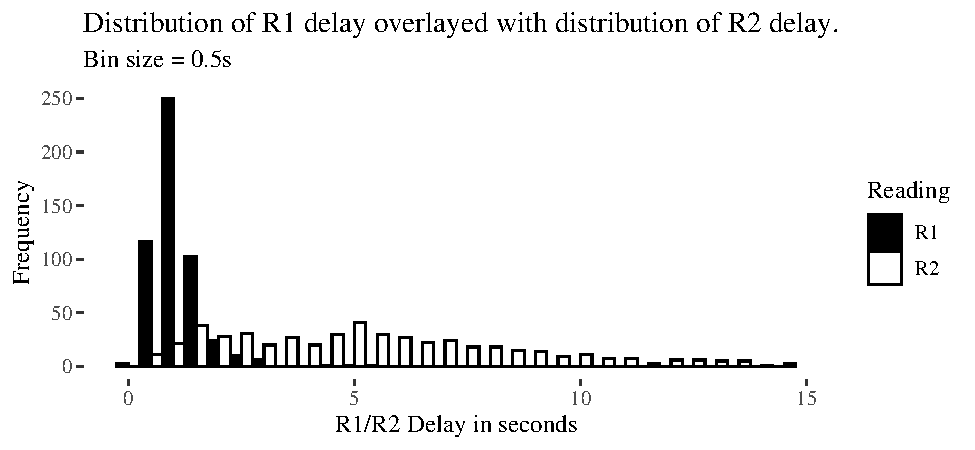
\includegraphics{4-results_files/figure-latex/delayComparison-1.pdf}
\caption{\label{fig:delayComparison}Distributions of R1 delay and R2 delay}
\end{figure}

As a way of analyzing the protocol, and the extent to which participants performed as expected, participants were categorized based on their median R1 delay. In what follows, a fast median R1 delay was shorter than or equal to 0.9s, and a slow one was longer than 1.05s, resulting in 12 participants per category. Ten participants had R1 delays between those values, categorized as ``normal,'' and set aside. The calculations for categorizing participants were done over Reading 1 of experimental items (n = 489). Note that while R1 delay category (i.e., fast or slow) is a property of R1 delay, data for both readings is nonetheless explored within these categories.

\begin{figure}
\centering
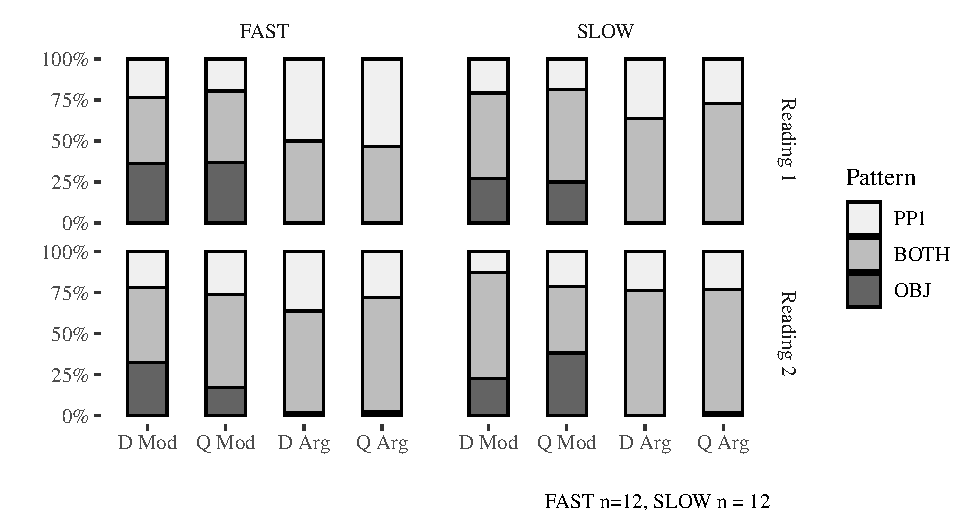
\includegraphics{4-results_files/figure-latex/facet-1.pdf}
\caption{\label{fig:facet}Plot of pattern proportions as a function of sentence type.}
\end{figure}

\begin{table}[t]

\caption{\label{tab:r2split}Break pattern by sentence type and R1 delay category.}
\centering
\begin{tabular}{cccc>{}c|cccc}
\toprule
\multicolumn{1}{c}{ } & \multicolumn{4}{c}{FAST (n=12)} & \multicolumn{4}{c}{SLOW (n=12)} \\
\cmidrule(l{3pt}r{3pt}){2-5} \cmidrule(l{3pt}r{3pt}){6-9}
  & D Arg & D Mod & Q Arg & Q Mod & D Arg & D Mod & Q Arg & Q Mod\\
\midrule
\addlinespace[0.3em]
\multicolumn{9}{l}{\textbf{Reading 1}}\\
\hspace{1em} & 46.5\% & 50.0\% & 43.5\% & 40.4\% & 72.9\% & 63.8\% & 56.2\% & 52.1\%\\
\cmidrule{2-9}
\multirow{-2}{*}{\centering\arraybackslash BOTH} & 20 & 24 & 20 & 19 & 35 & 30 & 27 & 25\\
\cmidrule{1-9}
\hspace{1em} & 0.0\% & 0.0\% & 37.0\% & 36.2\% & 0.0\% & 0.0\% & 25.0\% & 27.1\%\\
\cmidrule{2-9}
\multirow{-2}{*}{\centering\arraybackslash OBJ} & 0 & 0 & 17 & 17 & 0 & 0 & 12 & 13\\
\cmidrule{1-9}
\hspace{1em} & 53.5\% & 50.0\% & 19.6\% & 23.4\% & 27.1\% & 36.2\% & 18.8\% & 20.8\%\\
\cmidrule{2-9}
\multirow{-2}{*}{\centering\arraybackslash PP1} & 23 & 24 & 9 & 11 & 13 & 17 & 9 & 10\\
\cmidrule{1-9}
\addlinespace[0.3em]
\multicolumn{9}{l}{\textbf{Reading 2}}\\
\hspace{1em} & 69.8\% & 61.7\% & 56.5\% & 45.7\% & 75.0\% & 76.6\% & 40.4\% & 64.6\%\\
\cmidrule{2-9}
\multirow{-2}{*}{\centering\arraybackslash BOTH} & 30 & 29 & 26 & 21 & 36 & 36 & 19 & 31\\
\cmidrule{1-9}
\hspace{1em} & 2.3\% & 2.1\% & 17.4\% & 32.6\% & 2.1\% & 0.0\% & 38.3\% & 22.9\%\\
\cmidrule{2-9}
\multirow{-2}{*}{\centering\arraybackslash OBJ} & 1 & 1 & 8 & 15 & 1 & 0 & 18 & 11\\
\cmidrule{1-9}
\hspace{1em} & 27.9\% & 36.2\% & 26.1\% & 21.7\% & 22.9\% & 23.4\% & 21.3\% & 12.5\%\\
\cmidrule{2-9}
\multirow{-2}{*}{\centering\arraybackslash PP1} & 12 & 17 & 12 & 10 & 11 & 11 & 10 & 6\\
\bottomrule
\end{tabular}
\end{table}

There is a statically significant difference between the number of cases where both breaks were produced across the fast (44) vs.~slow (65) category for Reading 1 (\(\chi\)\textsuperscript{2}(1) = 4.05, p \textless{} 0.05), but not for Reading 2 (\(\chi\)\textsuperscript{2}(1) = 1.86, p = 0.17). There was also a statically significant difference in the occurrence of both breaks across PP2 Status for Reading 2 in the slow R1 delay category (\(\chi\)\textsuperscript{2}(1) = 3.97, p \textless{} 0.05), but comparisons across other factors represent in Table \ref{tab:arg} did not yield significant results. The maximum count per cell in the table is 96 (12 participants per category, 8 items per PP2 Status), ignoring missing items.

\begin{table}[!h]

\caption{\label{tab:arg}Occurrence of both breaks as a function of Reading, PP2 Status, and R1 Delay Category.}
\centering
\begin{tabular}{lrr}
\toprule
  & Reading 1 & Reading 2\\
\midrule
\addlinespace[0.3em]
\multicolumn{3}{l}{\textbf{Mod}}\\
\hspace{1em}FAST & 39 & 47\\
\hspace{1em}SLOW & 52 & 50\\
\addlinespace[0.3em]
\multicolumn{3}{l}{\textbf{Arg}}\\
\hspace{1em}FAST & 44 & 59\\
\hspace{1em}SLOW & 65 & 72\\
\bottomrule
\end{tabular}
\end{table}

In cases where R1 delay was small, readers were more likely to produce only one break than if R1 delay was fast. A possible explanation is that the slow starters were more prone to hesitation in general, or perhaps were using both the delay time and their extra break time to look ahead. The significant effect of PP2 Status for slow starters in Reading 2 could be due to the slow starters not fully understanding the Arg sentences prior to Reading 2, thus increasing their likelihood of hesitation.

\hypertarget{discussion-of-prosodic-break-patterns}{%
\section{Discussion of prosodic break patterns}\label{discussion-of-prosodic-break-patterns}}

Throughout the analysis of break patterns, PP2 Status was the most robust predictor of OBJ and PP1 break occurrence and their relative strengths. The OBJ break was more frequent and more frequently dominant for sentences with a PP2 that was an argument than those with a PP2 that could be a modifier; inversely, the PP1 break was more frequent and more frequently dominant for sentences with a PP2 that was interpretable as a modifier than those with a PP2 that was an argument.

Essentially, the expected patterns can be described as in (46) and (47), where \% represents a robust prosodic break, and @ represents a weaker break or no break.

\begin{enumerate}
\def\labelenumi{(\arabic{enumi})}
\setcounter{enumi}{45}
\item
  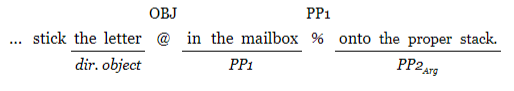
\includegraphics{breakpat1.png}
\item
  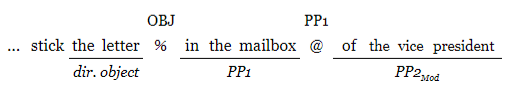
\includegraphics{breakpat2.png}
\end{enumerate}

This is supportive of \emph{hypothesis 1} presented in the introduction; and, in fact, of a broader formulation of it. Essentially, it's predicted that the PP1 break will more often be dominant for Arg cases, while the OBJ break will more often be dominant for Mod cases, because those break locations correspond to the position where the branching direction in the syntactic tree changes.

\emph{Hypothesis 1} \hfill\linebreak
Argument attachment of PP2 is marked by a dominant prosodic break between PP1 and PP2.

\emph{Broadened hypothesis 1} \hfill\linebreak
A change in branching direction is marked by a prosodic break.

A change in branching direction is taken to mean the closure of the preceding phrase and attachment into its parent node; in this case, either the closure of PP1 and the attachment off PP2 into the VP or the closure of the object NP and attachment of PP1 into the VP.

That Reading 2 is a significant predictor in 3 of the 4 analyses where its inclusion is possible supports, at least provisionally, hypothesis 2 and 3.

\emph{Hypothesis 2} \hfill\linebreak
A first reading of a sentence where PP2 is a goal argument will exhibit less natural prosody (more hesitation at and within the PP2 region) than:
* A first reading of a sentence where PP2 is a modifier
* A second reading of a sentence where PP2 is a goal argument

It is difficult to know whether a given reading represents more or less natural prosody, but given that there is a difference between readings, it seems most likely that Reading 2 is the more natural of the two since it represents a considered reading, rather than a hurried one. \emph{Hypothesis 2-3} are supported only if that assumption is accepted.

\emph{Hypothesis 3} \linebreak
A first reading of a sentence with an argument-PP2 will more often be produced with prosodic structure that represents an implausible or ungrammatical parse of the string (PP2 incorrectly attached as a modifier), whereas a second reading sentence will more often be pronounced with the prosodic structure that represents the intended parse (argument attachment of PP2).

\begin{enumerate}
\def\labelenumi{(\arabic{enumi})}
\setcounter{enumi}{47}
\tightlist
\item
  \emph{Hypothesis 4} \linebreak
  Reading 1 of a declarative sentence with an argument-PP2 will exhibit less natural prosody (more hesitation at and after the disambiguating region) and be more likely to be produced with prosodic structure that represents an implausible or ungrammatical parse of the string than a Reading 1 of an interrogative sentence with an argument-PP2.
\end{enumerate}

It is surprising that the effect of PP2 Status is generally lessened in Reading 2 when compared to Reading 1, but this can likely be explained as an epi-phenomenon. There is no way to distinguish between prosodic breaks that are intentional and syntactically motivated as compared to those that represent hesitation, a need for a breath, or other factors. It is likely that some of the effect of PP2 Status is actually an increase in hesitation after PP1, and therefore more or longer pauses at that position, which is mitigated in Reading 2. If some readers are, in general, simply producing a break after every phrase, but happen to produce what is perceived as a dominant break after PP1 for the Arg sentences when they are confused, that effect of PP2 Status will go away in Reading 2 once they have had time to figure the sentence out. This might mean that the noise caused by readers that are simply breaking phrase-by-phrase is actually amplified in Reading 2.

That a prosodic break also frequently occurs between phrases when there is no change in branching direction is mitigated somewhat by the fact that such breaks are usually weaker than the ones that do represent such a change. It is likely that these breaks are actually there for non-syntactic reasons; the end of a phrase represents a reasonable time for the speaker to take a breath or pause briefly for processing reasons. It is also likely that some readers are simply producing a break after each phrase.

Speech act is a significant predictor of PP1 break dominance (β=0.31, std. error = 0.15, p \textless{} 0.05)., but not of any of the other outcomes. It's plausible that the PP1 break is more likely to be dominant in questions than in declaratives because of the need to begin the sentence final rise of question intonation. That there is never an interaction between Speech Act and PP2 Status is discouraging for the hypothesis that it's the \emph{prosody} of questions that make the Arg cases seem easier in the interrogative cases compared to the declarative.

\hypertarget{irt}{%
\section{Inter-reading time}\label{irt}}

Inter-reading time is the amount of time after the completion of Reading 1 and before the beginning of phonation of Reading 2. The details of how this was measured and defined can be found in section \ref{method-irt}. IRT is meant to be a measure to some extent of how much difficulty the reader has in processing a given sentence. If a reader spends more time studying a sentence prior to reading it aloud a second time, the IRT will be longer, and I take that has an indicator of processing load.

Importantly, IRT is a measure across pairs of recordings (Reading 1/Reading 2), so the number of data analyzed in this section are half as many as those in the prosody analyses.

\hypertarget{irtDis}{%
\subsection{Data cleanup}\label{irtDis}}

IRTs below 0.25s (2) and above 25.0s (5) were assumed to be implausible and omitted. Experimental data were then Winsorized by participant to bring data below the 2.5\% and above the 97.5\% threshold to the value at those thresholds. The resulting measure is referred to as wIRT and is distributed as shown in figure \ref{fig:wIRT} (n = 489).

\begin{figure}
\centering
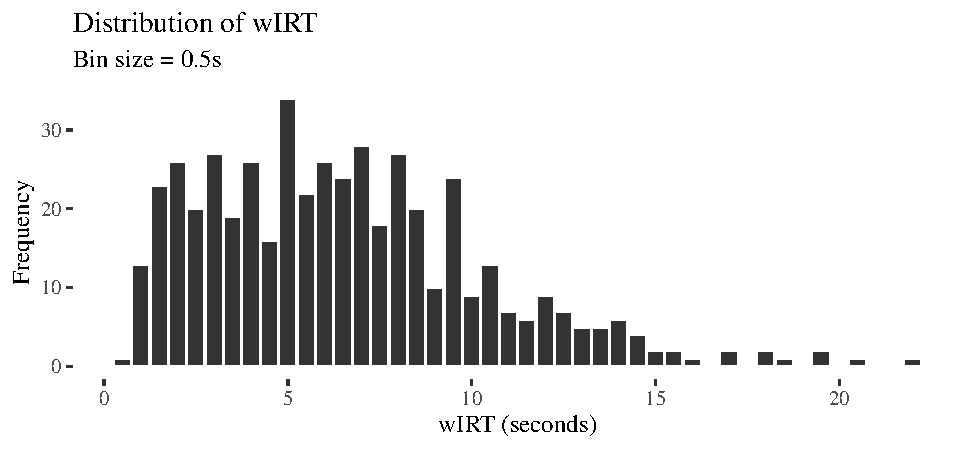
\includegraphics{4-results_files/figure-latex/wIRT-1.pdf}
\caption{\label{fig:wIRT}Distribution of wIRT.}
\end{figure}

Overall mean for wIRT was 6.5s (sd = 3.8). The longest wIRT was 22.2s and the shortest was 0.7s. Median wIRT was 6.1s.

\hypertarget{irtRes}{%
\subsection{Analysis of IRT data}\label{irtRes}}

Figure \ref{fig:interactionplot} shows the mean IRT as a function of sentence type.

\begin{figure}
\centering
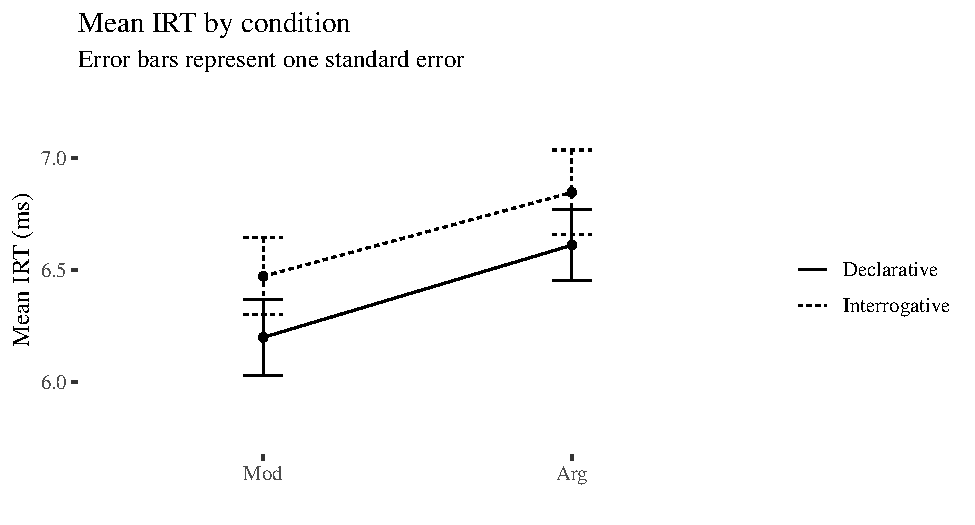
\includegraphics{4-results_files/figure-latex/interactionplot-1.pdf}
\caption{\label{fig:interactionplot}Mean IRT as a function of sentence type.}
\end{figure}

The two slopes are only very slightly divergent. Notably, both Speech Act and PP2 Status appear to have main effects on wIRT, with interrogatives attracting longer (6.7s) IRTs than declaratives (6.4s), and sentences with argument PP2s having substantially longer IRTs (6.7s) than those with modifier PP2s (6.3s).

Regression models support the observations above. All models discussed include random intercepts for participant and item. Models with random slopes for fixed effects all resulted in singular fits and so random slopes were not included.

By hypothesis, the best model for predicting IRT should be one with fixed effects of Speech Act and PP2 stats and the interaction between them. This model is shown in table \ref{tab:hyp}.

\begin{table}[!h]

\caption{\label{tab:hyp}Linear mixed effects regression model predicting wIRT by sentence type with interaction term (FULL).}
\centering
\begin{tabular}{rcccrcccrcccrccc}
\toprule
FULL MODEL & Estimate & Std. Error & p\\
\midrule
D Mod (Intercept) & 6.32 & 0.59 & < 0.001\\
Q & 0.29 & 0.30 & 0.34\\
Arg & 0.42 & 0.30 & 0.17\\
Q x Arg & 0.08 & 0.43 & 0.85\\
\bottomrule
\end{tabular}
\end{table}

Of the models with subset(s) of these predictors, the best (the model with the lowest AIC) was the one without the interaction term, shown in table 4.14.

\begin{table}[!h]

\caption{\label{tab:redirt}Linear mixed effects regression model predicting wIRT by sentence type (REDUCED).}
\centering
\begin{tabular}{rcccrcccrcccrccc}
\toprule
REDUCED MODEL & Estimate & Std. Error & p\\
\midrule
D Mod (Intercept) & 6.30 & 0.58 & < 0.001\\
Q & 0.33 & 0.21 & 0.12\\
Arg & 0.46 & 0.21 & < 0.05\\
\bottomrule
\end{tabular}
\end{table}

The difference between the reduced and full model was not statistically significant (AIC\textsubscript{FULL}=9103.5, AIC\textsubscript{REDUCED}=9101.6, \(\chi^2\)(1)=0.04, p \textgreater{} 0.8).

\hypertarget{pp2h}{%
\subsection{On PP2 heads}\label{pp2h}}

As mentioned in the items description (section 3.4), half of the items used \emph{of} for the head of PP2 in the Mod cases, while half used \emph{from.} In the Arg condition, half used \emph{into} and half used \emph{onto} to head PP2. An analysis that looks at the identity of the PP2 head found that while \emph{into} and \emph{onto} do not behave differently, \emph{of} and \emph{from} do. Starting from a maximally complex model that included the lexical identity of the matrix verb, the construction verb, the head of PP1, and the head of PP2, as well as Speech Act and PP2 Status, the model that best predicted wIRT was one that is essentially the same as the reduced model just reported (i.e., with Speech Act and PP2 Status as predictors), except it substitutes the lexical identity of the PP2 head for PP2 Status, with \emph{into} and \emph{onto} collapsed into one level used as the reference level (intercept).

\begin{table}[!h]

\caption{\label{tab:pp2hd}Linear mixed effects regression model predicting wIRT by Speech Act and PP2 head.}
\centering
\begin{tabular}{rcccrcccrcccrccc}
\toprule
PP2 head model & Estimate & Std. Error & p\\
\midrule
D into/onto (Intercept) & 6.76 & 0.58 & < 0.001\\
Q & 0.32 & 0.21 & 0.13\\
from & -0.08 & 0.27 & 0.77\\
of & -0.84 & 0.27 & < 0.01\\
\bottomrule
\end{tabular}
\end{table}

Sentences where PP2 was headed by \emph{from} typically had wIRTs that were 0.84s faster than sentences where PP2 was headed by \emph{into}/\emph{onto}; when the PP2 head was \emph{from} wIRT was only 0.08s faster than for \emph{into}/\emph{onto}, a difference that is not statistically significant (p \textgreater{} 0.7).

\hypertarget{discussion-of-irt-results}{%
\section{Discussion of IRT results}\label{discussion-of-irt-results}}

It is clear from the above that argument PP2s (ones headed by \emph{into}/\emph{onto}) result in longer wIRT measures. It also appears that interrogativity increases wIRT to a lesser extent, regardless of the PP2 Status. Because the interaction between the two factors is not a significant predictor of wIRT, we are left to assume that wIRT does not represent a behavioral reflex of the intuition that interrogativity makes difficult to process PP2-attachment ambiguities easier.

The difference between \emph{from} and \emph{of} PP2s is potentially a source of noise. The \emph{from} sentences are less clearly disambiguated than the \emph{of} sentences. Where (49) has only one reading, (50) has another possible reading, albeit somewhat implausible: i.e., we could imagine that in (49) \emph{from her brother-in-law} modifies \emph{the cookies}, while in (4) \emph{of the minivan} cannot modify \emph{the bicycle}.

\begin{enumerate}
\def\labelenumi{(\arabic{enumi})}
\setcounter{enumi}{48}
\tightlist
\item
  She had intended to put the bicycle on the roof rack of the minivan.
\item
  She had decided to cram the cookies in the basket from her brother-in-law.
\end{enumerate}

This lingering ambiguity could have increased wIRT somewhat because the reader, given unlimited time, spent some of that time noticing and then eliminating that possible reading. The difference here can be explained by once again making an appeal to structural parsing vs.~structural association: if we imagine that a \emph{from} PP is associated rather than parsed, the reader is free to consider other possible interpretations. Because \emph{of} can be seen as less a preposition and more a functional head, it stands to reason that it would be treated different, as something that must be parsed immediately, i.e., that \emph{from her brother-in-law} is modifying, where \emph{of the minivan} is in some sense more argument-like. This is similar to an established observation about what constituents pro-forms can stand in for: (51) is ungrammatical, but (52) is fine; the same holds for (53) where \emph{to Fred} is an argument, compared to (54) where \emph{for Fred} is a modifier.

\begin{enumerate}
\def\labelenumi{(\arabic{enumi})}
\setcounter{enumi}{50}
\item
  \(*\) I saw the student of physics and the one of chemistry arguing with each other.
\item
  \(\checkmark\) I saw the student from Texas and the one from Maine arguing with each other.
\item
  \(*\) Mary gave a book to Fred and did so to John, too.
\item
  \(\checkmark\) Mary signed a book for Fred and did so for John, too.
\end{enumerate}

It could also be a simpler explanation: the fact that \emph{of} is only two characters, whereas \emph{from} and \emph{into}/\emph{onto} are all four characters, participants may have recognized a pattern, wherein they could be sure that a two-character PP2 head meant the sentence did not have the difficult properties of some of the ones with four-character PP2 heads (most notably the \emph{into}/\emph{onto} cases), and eliminated some of the needed study time.

\hypertarget{qslow}{%
\subsection{The processing cost of interrogativity}\label{qslow}}

It is worth taking note of the fact that the mean wIRT for interrogative versions (6.7s) of the experimental sentences in the reported study was longer than for the declaratives (6.4s). While this finding was not statistically significant, Peckenpaugh (2016) found that whole-sentence silent reading times for interrogatives were longer than for declaratives; and Mehler (1963) provided a very early report of the processing cost of interrogativity: a so-called kernel sentence, i.e., a simple declarative, was easier to recall verbatim than was a number of sentences that he considered to be syntactic transformations of that kernel sentence (K): negative (N), polar question (Q), passive (P), and combinations thereof: NQ, NP, QP and NPQ. Mehler found that accurate recall was more frequent for K sentences (300/460, 65.2\%) than for the other sentences types, with interrogatives (210/460, 45.7\%) being recalled accurately at a lower rate than the two other individual transformations (234/460, 50.9\% for N; 243/460, 52.8\% for P).

The filler sentences in this study were designed in two versions, interrogative (Q) and declarative (D), so as to provide a diagnostic of the interrogative effect on IRT independent of the experimental question. A linear mixed effects regression model predicting wIRT for filler items by interrogativity with crossed random intercepts (participant and item) found that wIRT is increased by 0.4s for interrogatives (std. error = 0.2; p \textless{} 0.05); declaratives had a mean wIRT of 6.2s, while interrogatives had a mean wIRT of 6.6s. Half of the fillers had a sequence of two PPs at the end to mirror the experimental items: a model predicting wIRT by the presence of those PPs found minimal effect on wIRT (β=0.01, std. error = 0.22, p = 0.96).

Interrogative status itself appears to increase the time needed for participants to feel they have satisfactorily studied a sentence in order to read it aloud correctly. This is consistent with the Mehler (1963) and Peckenpaugh (2016) findings that interrogatives are in some way more complicated or difficult than declaratives.

\clearpage

\hypertarget{general-discussion}{%
\chapter{General discussion}\label{general-discussion}}

This chapter will review the questions motivating this study and discuss the extent to which those questions are answered, or not. It will then go on to develop further questions, and propose further studies to explore those new questions and the ones left unanswered here. Finally, it will summarize the findings and the current standing of this area of research.

Recall that the primary motivation for this study was the possibility that PP-attachment garden paths are easier to understand for speakers of American English when presented in the interrogative, as opposed to the declarative. In Section \ref{obs}, a distinction was made between the intuition first outlined in Peckenpaugh (2016) and the current hypothesis. For terminological clarity, recall the definitions originally given in \ref{obs}:

\begin{enumerate}
\def\labelenumi{(\arabic{enumi})}
\setcounter{enumi}{54}
\item
  \emph{The 2016 intuition:} Certain pragmatically disambiguated prepositional phrase (PP) attachment ambiguities which are difficult to parse in the declarative are less difficult to parse when presented as yes-no interrogatives (e.g., Jed crammed the newspapers under the sofa in the trashcan) (cf.~Peckenpaugh (2016)).
\item
  \emph{The current hypothesis:} The intuition may be extensible to PP attachment ambiguities that are syntactically disambiguated in addition to those that are pragmatically disambiguated (e.g., Had he planned to cram the paperwork {[}\textsubscript{PP1} in the drawer{]} {[}\textsubscript{PP2} into his briefcase{]}?).
\end{enumerate}

The goal of this study was to establish whether there is evidence for (56), and to explore the implications of those findings for possible explanations of (55).

\hypertarget{behavioral-correlate-for-the-2016-intuition-and-the-current-hypothesis}{%
\section{Behavioral correlate for the 2016 intuition and the current hypothesis?}\label{behavioral-correlate-for-the-2016-intuition-and-the-current-hypothesis}}

\comment{section title updated}

Ultimately, no evidence has been found to support the current hypothesis, that the intuition can be extended to syntactically disambiguated sentences. Mixed-effect regression analyses were not able to detect statistical significance for the interaction between Speech Act and PP2 Status. This does not, of course, negate the intuition; it simply means that we have not yet found a behavior that can be said with certainty to correspond to that intuition. Future research should pursue the possibility that IRT (Inter-reading Time) is not the ideal measure for detecting any behavioral correlate of the processing difference for PP-attachment garden paths between interrogatives and declaratives.

\hypertarget{on-possible-explanations-for-the-intuition}{%
\section{On possible explanations for the intuition}\label{on-possible-explanations-for-the-intuition}}

This section looks at the evidence for and against some of the possible explanations for the intuition reported in Peckenpaugh (2016).

\hypertarget{prep}{%
\subsection{A prosodic account}\label{prep}}

The prosodic phrasings produced by participants in this study varied systematically by PP2 Status \added{(Arg vs. Mod, where Arg is the garden path case)}. This is an interesting finding in and of itself, adding to the growing literature that shows a link between syntactic structure and prosodic phrasing. A possible explanation for the intuitive effect of interrogativity on parsing garden paths is provided in the work by Bader (1998). Bader demonstrates that it is easier to recover \added[id=JDF]{from} a \added[id=JDF]{failed} parse that ``behave{[}s{]} alike prosodically'' to a given failed parse, because the reanalysis does not require prosodic reconstruction and only the syntax needs to be repaired. In the case of the \added{2016} intuition\deleted[id=JDF]{this study is concerned with}, this would mean that if sentences were more \added[id=JDF]{prosodically} similar across the Arg vs.~Mod PP2 Status in the interrogative than in the declarative, the intuit\replaced[id=JDF]{ed}{ive} reduction in difficulty of reanalysis would naturally follow. \added{This assumes, of course, that the 2016 iuntuition is eventually confirmed, despite the inconclusive results of} Peckenpaugh (2016).

The findings of \replaced[id=JDF]{the current}{this} study show that there is no one-to-one mapping between prosodic structure and the four sentence types \replaced[id=JDF]{test in this}{defined by the design of the} study (Q Arg, D Arg, Q Mod, D Mod). Rather, \added[id=JDF]{for each Sentence Type,} \deleted[id=JDF]{there are} gradient differences in occurrence \replaced[id=JDF]{of}{for} each pattern for a given sentence type \added[id=JDF]{were observed}. \added[id=JDF]{Recall that a break after the direct object is referred to as the object break (OBJ), and one after PP1 is referred to as the PP1 break (PP1).} Table \ref{tab:combobr} shows the distribution of the possible \deleted[id=JDF]{simple} break patterns (PP2 break only, OBJ break only, or both breaks, with the negligible number of cases of neither break omitted) as a function of sentence type for Reading 2 only. These data are a subset of the data reported in Section \ref{bbr} Table \ref{tab:bothbreaks}.

\begin{table}[!h]

\caption{\label{tab:combobr}Percent occurrence of break patterns in Reading 2 as a function of sentence type.}
\centering
\begin{tabular}{>{\bfseries}lcccc}
\toprule
\multicolumn{1}{c}{ } & \multicolumn{2}{c}{Mod} & \multicolumn{2}{c}{Arg} \\
\cmidrule(l{3pt}r{3pt}){2-3} \cmidrule(l{3pt}r{3pt}){4-5}
  & D & Q & D & Q\\
\midrule
OBJ only & 14.8 & 25.6 & 27.0 & 25.8\\
PP1 only & 54.1 & 43.0 & 72.1 & 71.7\\
Both breaks & 31.1 & 31.4 & 0.8 & 2.5\\
\bottomrule
\end{tabular}
\end{table}

While there is a larger drop in the number of utterances with both breaks from \replaced{Arg}{+GP} to \replaced{Mod}{-GP} for questions \textbackslash{}added{[}id=JDF{]}\{(71.7\% - 43.0\%)\} than for declaratives \textbackslash{}added{[}id=JDF{]}\{(72.1\% - 54.1\%)\}, the opposite is true for the pattern with a PP1 break by itself \textbackslash{}added{[}id=JDF{]}\{(25.8\% - 25.6\% vs.~27.0\% - )\}. There is an argument to be made that the OBJ break\replaced{in the Arg versions}{, which does not correspond to a change in syntactic branching direction for any version of the sentences,} is \added{not a true prosodic break but} a hesitation \deleted{rather than a break,} due to a moment of confusion or \replaced{for length reasons}{perhaps simply a need to breathe}.

\comment{more on length...}

\replaced{If the prosodic structures}{To be more explicit, for this explanation to work, the prosodic structures} in (57), (58), (59) and (60) \replaced{are assumed to be ideal, then an explanation for the 2016 intuition (and by extension, the same explantion for syntactically disambiguated cases) presents itself.}{would likely be the ones considered "correct" or most common for a the declarative versions.} The symbol ``\%'' is being used to represent a prominent prosodic break \added{in} (57) and (58).

\begin{enumerate}
\def\labelenumi{(\arabic{enumi})}
\setcounter{enumi}{56}
\tightlist
\item
  \emph{D Arg}: He had crammed {[}\textsubscript{OBJ} the newspapers{]} {[}\textsubscript{PP1} under the sofa{]} \% {[}\textsubscript{PP2} into the trashcan{]}.
\item
  \emph{D Mod}: He had crammed {[}\textsubscript{OBJ} the newspapers{]} under the sofa in the guestroom.
\end{enumerate}

\repalced{The two declarative versions differ from each other in that the Arg case is ideally pronounced with a major break after *under the sofa* to mark the argument attachment of PP2; whereas in the Mod case does not require that break in the ideal pronunciation (though it may sometimes occur for length reasons).}{The prosodic structure of @dhi does not mandate any major break, because there is no change in syntactic branching directory and no other reason to mandate a break there.} That is, the PP1 break differentiates the two syntactic structures and signals the attachment site of PP2 in the Arg case.

For the interrogatives, though, this contrast is obscured by the need to apply a rising prosodic contour over the final nuclear accent in the sentence: i.e., PP2, resulting in not a change in syntactic branching direction, but the anticipation of a tonal change, which might sound very similar to a prosodic break. The symbol ``\(\Uparrow\)'' indicates the start of the rising contour.

\begin{enumerate}
\def\labelenumi{(\arabic{enumi})}
\setcounter{enumi}{58}
\tightlist
\item
  \emph{Q Arg}: Had he crammed {[}\textsubscript{OBJ} the newspapers{]} {[}\textsubscript{PP1} under the sofa{]} \% {[}\textsubscript{PP2} into the \(\Uparrow\) trashcan{]}?
\item
  \emph{Q Mod}: Had he crammed {[}\textsubscript{OBJ} the newspapers{]} {[}\textsubscript{PP1} under the sofa {[}\textsubscript{PP2} in the \(\Uparrow\) guestroom{]}{]}?
\end{enumerate}

The critical issue here is that in (60), the absence of a syntactically-motivated break might be obscured by the hesitation necessitated by preparing to start the final-rising contour of a question two words later. It's not impossible that the need to make the mechanical preparation necessary to execute a rising contour could result in a hesitation or pause at the preceding syntactic juncture most welcoming to it, the PP1 break position. \added{While in} (60) \added{PP2 is a subconstituent of PP1, and so the final phrase is actually PP1, the final nuclear accent still falls on the NP within PP2, and so final high rise is anchored to the same phrase in both interrogative versions (Arg and Mod).}

If the PP1 break is treated as the main indicator of the prosodic structure, then the larger difference across PP2 Status for declaratives (12.2\%) than for interrogatives (0.2\%) does, though perhaps weakly, leave open the door for the Bader (1998) style explanation of the intuition. Ultimately, though, logistic regression models showed no significant effect of the interaction between Speech Act and PP2 Status, so it is safest to assume that this difference is just noise, and that the explanation for the intuition is not prosodic.

\hypertarget{a-processing-illusion}{%
\subsection{A processing illusion}\label{a-processing-illusion}}

\added[id=JDF]{If the above explanation proves not to be viable in subsequent study,} \replaced[id=JDF]{a}{A}nother possibility to consider is that the intuition itself is illusory in nature, i.e., it is not the case that interrogative PP-attachment garden paths (\added[id=JDF]{either} pragmatically or syntactically disambiguated) are easier to parse than declarative ones\added{,} but only appear to be so. \deleted{Perhaps the Q Arg sentences are not actually easier to parse, but \added{only} appear to be}\relaced{. B}{, b}ecause the added complexity of the interrogative version is distracting the reader with a different sort of difficulty. It may be that \added[id=JDF]{readers} are being distracted by the processing cost of interrogativity, and thereby are less sensitive to the cost of reanalysis. While the parser is struggling with two additive increases to complexity as compared to D Mod sentences (i.e., Arg PP2 Status and interrogative context) the reader is aware only of the more immediately obvious difference, that of interrogativity, and fails to \deleted[id=JDF]{consciously} notice the structural reanalysis that the parser is undertaking.

\hypertarget{confound}{%
\section{Conclusions}\label{confound}}

In this section, I will discuss some of the \added[id=JDF]{potential} issues \replaced[id=JDF]{raised by}{with} the current study, and what I see as fruitful avenues for future \replaced[id=JDF]{researc}{study}.

\hypertarget{inter-item-reading-time-irt-findings}{%
\subsection{Inter-item reading time (IRT) findings}\label{inter-item-reading-time-irt-findings}}

\added{A number of interesting findings are supported by IRT and the Double Reading paradigm used in the current study.}

While IRT did not detect a behavioral correlate of the motivating intuition for this study, it did show a robust effect of PP2 Status \added[id=JDF]{(Arg vs. Mod)}, indicating that it may yet be a useful diagnostic for parsing difficulty \added[id=JDF]{in general}.

The IRT data reported also supported prior findings that interrogatives are \added{generally} slower \added[id=JDF]{to process} or more difficult to comprehend than \replaced[id=JDF]{related}{similar} declarative sentences, \added[id=JDF]{as noted by} Mehler (1963) and Peckenpaugh (2016) \added[id=JDF]{(see Section} \ref{qslow}\added[id=JDF]{)}. .

The fact that reading (Reading 1 vs.~Reading 2) frequently had an effect on prosodic phrasing also supports the finding of Fodor et al. (2019) that \added[id=JDF]{"cold" and previewed readings have different properties and can provide different sorts of evidence, thus} item preview should be tightly controlled \replaced[id=JDF]{and documented}{when one is studying prosodic structure}.

\hypertarget{future-work}{%
\subsection{Future work}\label{future-work}}

Some future studies that could further this line of research are outlined below.

\hypertarget{embedded-questions}{%
\subsubsection{Embedded questions}\label{embedded-questions}}

The explanation for the intuition that PP-attachment garden paths are less difficult to parse in interrogatives than in declaratives must either be prosodic, or else semantic/pragmatic. It seems very unlikely that the minor syntactic difference across the two sentence types (i.e., subject-auxiliary inversion) could be the reason for a difference in perceived ease of understanding. It is either the difference in the intonational contour between the two sentences types, or else it is something about the meaning or meta-linguistic difference between interrogatives and declaratives. The study just reported has shown evidence that the intuition can not easily be explained entirely by the prosodic differences between questions and declaratives; the possibility remains weakly at best. It seems that most important next step in explaining the aforementioned intuition would be to look at the same phenomenon in embedded questions vs.~embedded declarative clauses, where prosody would not be at play but the semantic/pragmatic differences should remain. For example:

\begin{enumerate}
\def\labelenumi{(\arabic{enumi})}
\setcounter{enumi}{60}
\item
  \emph{Em Q \replaced{Arg}{+GP}:} He asked her if she had decided to cram the old newspapers under the couch in the wastebasket.
\item
  \emph{Em Q \replaced{Mod}{-GP}:} He asked her if she had decided to cram the old newspapers under the couch in the guestroom.
\item
  \emph{Em D \replaced{Arg}{+GP}:} She told him that she had decided to cram the old newspapers under the couch in the wastebasket.
\item
  \emph{Em D \replaced{Mod}{-GP}:} She told him that she had decided to cram the old newspapers under the couch in the guestroom.
\end{enumerate}

The prosody of an embedded question, as in (61), does not differ from that of a sentence like (63); but, the semantic properties and some of the pragmatic properties of the embedded clause in (61) are the same as in the Q Arg sentences from the study just reported.

\begin{enumerate}
\def\labelenumi{(\arabic{enumi})}
\setcounter{enumi}{64}
\tightlist
\item
  Had she decided to crammed the old newspapers under the couch in the wastebasket?
\end{enumerate}

These stimuli could be used with ERP or eye-tracking methodology to see if parsing difficulty differs across the embedded clause's declarative vs.~interrogative nature. If a behavioral correlate of the intuition is found with embedded question stimuli, that would be strong evidence that the explanation is semantic or pragmatic rather than prosodic.

\hypertarget{hesitations-vs.-prosodic-breaks}{%
\subsection{Hesitations vs.~prosodic breaks}\label{hesitations-vs.-prosodic-breaks}}

An issue with the findings of this study is the difficulty in differentiating between syntactically-motivated prosodic breaks and hesitations. As shown by the reliability data reported in Section \ref{rel} illustrates, a linguistically trained judge will not necessarily be able to agree where breaks fall and which breaks are stronger, likely in large part because of the difficulty in differentiating between prosodic breaks and hesitations.

It is famously difficult to instrumentally describe a prosodic break, and there is no guarantee that examining the wave forms instrumentally would fare any better in making this distinction than the intuition of the judges. That said, it may be possible to distinguish the two sorts of breaks: it may be that boundary tones or segmental lengthening are typically not part of a hesitation break, but are a part of hesitation break, for example. No immediately apparent pattern is available, but it would be inordinately beneficial if one could be found.

In \ref{erp} I propose that an event-related potential paradigm might hold the key for distinguishing between the two.

\hypertarget{erp}{%
\subsubsection{Event-related potential (ERP) study}\label{erp}}

An event-related potential study of the phenomenon could provide a number of useful insights. It has been shown that the so-called closure-positive shift (CPS), an ERP component that is elicited by the presence of a prosodic break or a comma, is present even in silent reading. This has a number of important implications for research on the phenomena at hand.

For one, it provides a way to distinguish between a hesitation after PP1 and a true prosodic break; which is to say, a way to distinguish between an unencumbered reading with a prosodic break after PP1 and a garden-path effect that, in the study reported here, resulted in a hesitation at that point. An ERP measure time-locked to that position should show a CPS component when the reader successfully incorporates PP1 as a modifier of the object and then changes branching direction to incorporate PP2 as the goal argument; conversely, a reader who is experiencing a garden-path effect at that point should instead or additionally show a P600 component (Steinhauer (2003) found that the two components can be additive). If the participant were concurrently recorded reading the sentence aloud, definitive data could be created which could then be used to either train a linguist or perhaps a neural network to distinguish between hesitations (P600s) and prosodic breaks (CPSes). The trained model or linguist could then return to the recordings collect for this study and make definitive judgments regarding the nature of the breaks reported here, and clarify the results of this study.

It would also be useful to see if repeated readings of the same garden-path sentence reduces the P600; if so, is the rate of decay faster for interrogatives than declaratives? Such a phenomenon could be a correlate of the reported intuition.

\hypertarget{summary}{%
\section{Summary}\label{summary}}

In sum, the current study has not found evidence that supports the extension of the intuition over items that are syntactically disambiguated. It has found an effect on IRT of the garden path effect in both declarative and interrogative cases, and it has found an effect of Speech Act on the IRT for filler items. There are systematic differences in the way that the different sentence types are prosodically structured, but the correspondence between sentence type and prosodic pattern is gradient rather than categorical. It's possible that a Bader-esque account can explain the intuition, or that the intuition is illusory, or that the intuition is due to semantic or pragmatic factors. It is also possible that the intuition simply does not apply to syntactically disambiguated instances of the garden path in question to the extent that it can be detected in the measures reported here. Further study via behavioral, eye-tracking, or ERP methodology are likely to be fruitful in further understanding the phenomenon.

\singlespacing

\newpage

\hypertarget{appendix-appendices}{%
\appendix}


\hypertarget{appExp}{%
\chapter{Experimental items}\label{appExp}}

\begin{longtable}{ll}
\caption{\label{tab:unnamed-chunk-1}Experimental items in four versions}\\
\toprule
Version & Text\\
\midrule
\endfirsthead
\caption[]{\label{tab:unnamed-chunk-1}Experimental items in four versions \textit{(continued)}}\\
\toprule
Version & Text\\
\midrule
\endhead
\
\endfoot
\bottomrule
\endlastfoot
Q Arg & Had she decided to cram the cookies in the basket into her jacket pocket?\\
D Arg & She had decided to cram the cookies in the basket into her jacket pocket.\\
Q Mod & Had she decided to cram the cookies in the basket from her brother-in-law?\\
D Mod & She had decided to cram the cookies in the basket from her brother-in-law.\\
\addlinespace
Q Arg & Had she decided to put the child on the rocking horse onto the see-saw?\\
D Arg & She had decided to put the child on the rocking horse onto the see-saw.\\
Q Mod & Had she decided to put the child on the rocking horse from his parents?\\
D Mod & She had decided to put the child on the rocking horse from his parents.\\
\addlinespace
Q Arg & Had he decided to set the board games on the floor onto the card table?\\
D Arg & He had decided to set the board games on the floor onto the card table.\\
Q Mod & Had he decided to set the board games on the floor of the living room?\\
D Mod & He had decided to set the board games on the floor of the living room.\\
\addlinespace
Q Arg & Had he decided to stick the large check in the envelope into her wallet?\\
D Arg & He had decided to stick the large check in the envelope into her wallet.\\
Q Mod & Had he decided to stick the large check in the envelope from her church?\\
D Mod & He had decided to stick the large check in the envelope from her church.\\
\addlinespace
Q Arg & Had he intended to cram the paperwork in the drawer into his boss's desk?\\
D Arg & He had intended to cram the paperwork in the drawer into his boss's desk.\\
Q Mod & Had he intended to cram the paperwork in the drawer of his filing cabinet?\\
D Mod & He had intended to cram the paperwork in the drawer of his filing cabinet.\\
\addlinespace
Q Arg & Had he intended to put the bicycle on the roof rack into the garage?\\
D Arg & He had intended to put the bicycle on the roof rack into the garage.\\
Q Mod & Had he intended to put the bicycle on the roof rack of the minivan?\\
D Mod & He had intended to put the bicycle on the roof rack of the minivan.\\
\addlinespace
Q Arg & Had she intended to set the clothes in the hamper onto the dresser?\\
D Arg & She had intended to set the clothes in the hamper onto the dresser.\\
Q Mod & Had she intended to set the clothes in the hamper from his sister?\\
D Mod & She had intended to set the clothes in the hamper from his sister.\\
\addlinespace
Q Arg & Had she intended to stick the letter in the mailbox onto the proper stack?\\
D Arg & She had intended to stick the letter in the mailbox onto the proper stack.\\
Q Mod & Had she intended to stick the letter in the mailbox of the vice president?\\
D Mod & She had intended to stick the letter in the mailbox of the vice president.\\
\addlinespace
Q Arg & Had she planned to cram the stolen files in the wall-safe into a suitcase?\\
D Arg & She had planned to cram the stolen files in the wall-safe into a suitcase.\\
Q Mod & Had she planned to cram the stolen files in the wall-safe of their hideout?\\
D Mod & She had planned to cram the stolen files in the wall-safe of their hideout.\\
\addlinespace
Q Arg & Had she planned to put the jelly beans in the window onto a fancy dish?\\
D Arg & She had planned to put the jelly beans in the window onto a fancy dish.\\
Q Mod & Had she planned to put the jelly beans in the window of his candy store?\\
D Mod & She had planned to put the jelly beans in the window of his candy store.\\
\addlinespace
Q Arg & Had he planned to set the appetizers on the platter onto the buffet?\\
D Arg & He had planned to set the appetizers on the platter onto the buffet.\\
Q Mod & Had he planned to set the appetizers on the platter from his cousin?\\
D Mod & He had planned to set the appetizers on the platter from his cousin.\\
\addlinespace
Q Arg & Had he planned to stick the post-it note on the handout onto his notebook?\\
D Arg & He had planned to stick the post-it note on the handout onto his notebook.\\
Q Mod & Had he planned to stick the post-it note on the handout from the lecture?\\
D Mod & He had planned to stick the post-it note on the handout from the lecture.\\
\addlinespace
Q Arg & Had he wanted to cram the newspapers under the sofa into the wastebasket?\\
D Arg & He had wanted to cram the newspapers under the sofa into the wastebasket.\\
Q Mod & Had he wanted to cram the newspapers under the sofa from the thrift store?\\
D Mod & He had wanted to cram the newspapers under the sofa from the thrift store.\\
\addlinespace
Q Arg & Had he wanted to put the photo on the coffee table onto the mantelpiece?\\
D Arg & He had wanted to put the photo on the coffee table onto the mantelpiece.\\
Q Mod & Had he wanted to put the photo on the coffee table from his grandfather?\\
D Mod & He had wanted to put the photo on the coffee table from his grandfather.\\
\addlinespace
Q Arg & Had she wanted to set the textbooks on the top shelf into the file box?\\
D Arg & She had wanted to set the textbooks on the top shelf into the file box.\\
Q Mod & Had she wanted to set the textbooks on the top shelf of the book shelf?\\
D Mod & She had wanted to set the textbooks on the top shelf of the book shelf.\\
\addlinespace
Q Arg & Had she wanted to stick the golf clubs in the back room into the closet?\\
D Arg & She had wanted to stick the golf clubs in the back room into the closet.\\
Q Mod & Had she wanted to stick the golf clubs in the back room of their condo?\\
D Mod & She had wanted to stick the golf clubs in the back room of their condo.\\*
\end{longtable}

\newpage

\hypertarget{appFill}{%
\chapter{Filler items}\label{appFill}}

\begin{longtable}{ll}
\caption{\label{tab:unnamed-chunk-2}Filler items with trailing PPs}\\
\toprule
Version & Text\\
\midrule
\endfirsthead
\caption[]{\label{tab:unnamed-chunk-2}Filler items with trailing PPs \textit{(continued)}}\\
\toprule
Version & Text\\
\midrule
\endhead
\
\endfoot
\bottomrule
\endlastfoot
+PP D & He had intended to enter the expenses from the trip into a spreadsheet.\\
+PP Q & Had he intended to enter the expenses from the trip into a spreadsheet?\\
\addlinespace
-PP D & He had intended to do the work that the boss asked a coworker to do.\\
-PP Q & Had he intended to do the work that the boss asked a coworker to do?\\
\addlinespace
+PP D & He had intended to sell his collection of baseball cards from his childhood.\\
+PP Q & Had he intended to sell his collection of baseball cards from his childhood?\\
\addlinespace
-PP D & He had intended to replace the crackers he ate while he was house sitting.\\
-PP Q & Had he intended to replace the crackers he ate while he was house sitting?\\
\addlinespace
+PP D & She had planned to tell the student in private about his failing grade.\\
+PP Q & Had she planned to tell the student in private about his failing grade?\\
\addlinespace
-PP D & She had planned to finish preparing dinner while the guests were chatting.\\
-PP Q & Had she planned to finish preparing dinner while the guests were chatting?\\
\addlinespace
+PP D & She had planned to pack a ham sandwich on rye bread into her lunchbox.\\
+PP Q & Had she planned to pack a ham sandwich on rye bread into her lunchbox?\\
\addlinespace
-PP D & She had planned to build herself a new computer when she got her paycheck.\\
-PP Q & Had she planned to build herself a new computer when she got her paycheck?\\
\addlinespace
+PP D & She had wanted to complete the race for charity in record time.\\
+PP Q & Had she wanted to complete the race for charity in record time?\\
\addlinespace
-PP D & She had wanted to bring her son when she attended the next conference.\\
-PP Q & Had she wanted to bring her son when she attended the next conference?\\
\addlinespace
+PP D & She had wanted to find a rare butterfly on their hike in the rainforest.\\
+PP Q & Had she wanted to find a rare butterfly on their hike in the rainforest?\\
\addlinespace
-PP D & She had wanted to tell her friends that she was selling her vacation home.\\
-PP Q & Had she wanted to tell her friends that she was selling her vacation home?\\
\addlinespace
+PP D & She had decided to break the class into teams of six students each.\\
+PP Q & Had she decided to break the class into teams of six students each?\\
\addlinespace
-PP D & He had decided to do the needed repairs on the broken-down van himself.\\
-PP Q & Had he decided to do the needed repairs on the broken-down van himself?\\
\addlinespace
+PP D & She had decided to instruct the staff on proper etiquette for formal dining.\\
+PP Q & Had she decided to instruct the staff on proper etiquette for formal dining?\\
\addlinespace
-PP D & He had decided to advise that his newest patient seek a second opinion.\\
-PP Q & Had he decided to advise that his newest patient seek a second opinion?\\
\addlinespace
+PP D & He had forgotten to try the famous pastry in the restaurant of the fancy hotel.\\
+PP Q & Had he forgotten to try the famous pastry in the restaurant of the fancy hotel?\\
\addlinespace
-PP D & She had forgotten to report that the clerk was ignoring her request.\\
-PP Q & Had she forgotten to report that the clerk was ignoring her request?\\
\addlinespace
+PP D & He had forgotten to tack the pamphlet on hygiene onto the notice board.\\
+PP Q & Had he forgotten to tack the pamphlet on hygiene onto the notice board?\\
\addlinespace
-PP D & She had forgotten to lock the gate that was supposed to be kept closed.\\
-PP Q & Had she forgotten to lock the gate that was supposed to be kept closed?\\
\addlinespace
+PP D & She had meant to arrange the files in alphabetical order for her boss.\\
+PP Q & Had she meant to arrange the files in alphabetical order for her boss?\\
\addlinespace
-PP D & She had meant to write up the performance reviews to give her employees.\\
-PP Q & Had she meant to write up the performance reviews to give her employees?\\
\addlinespace
+PP D & She had meant to place a suggestion box onto the front desk of the clinic.\\
+PP Q & Had she meant to place a suggestion box onto the front desk of the clinic?\\
\addlinespace
-PP D & She had meant to try to get the program to run on the new operating system.\\
-PP Q & Had she meant to try to get the program to run on the new operating system?\\
\addlinespace
+PP D & He had needed to request some money from his father-in-law for the remodel.\\
+PP Q & Had he needed to request some money from his father-in-law for the remodel?\\
\addlinespace
-PP D & He had needed to upgrade his ticket when he changed his travel plan.\\
-PP Q & Had he needed to upgrade his ticket when he changed his travel plan?\\
\addlinespace
+PP D & He had needed to set the vegan cookies onto serving trays for the party.\\
+PP Q & Had he needed to set the vegan cookies onto serving trays for the party?\\
\addlinespace
-PP D & He had needed to beg to get his old job back when his investment failed.\\
-PP Q & Had he needed to beg to get his old job back when his investment failed?\\
\addlinespace
+PP D & He had remembered to add the section into the handboook for the meeting.\\
+PP Q & Had he remembered to add the section into the handboook for the meeting?\\
\addlinespace
-PP D & He had remembered to tell the office manager to order more coffee filters.\\
-PP Q & Had he remembered to tell the office manager to order more coffee filters?\\
\addlinespace
+PP D & He had remembered to move the gifts from the baby shower onto the bed.\\
+PP Q & Had he remembered to move the gifts from the baby shower onto the bed?\\
\addlinespace
-PP D & He had remembered to circulate the latest job posting his company had sent.\\
-PP Q & Had he remembered to circulate the latest job posting his company had sent?\\*
\end{longtable}

\newpage

\begin{longtable}{lll}
\caption{\label{tab:unnamed-chunk-3}Filler items with no trailing PPs}\\
\toprule
  & Version & Text\\
\midrule
\endfirsthead
\caption[]{\label{tab:unnamed-chunk-3}Filler items with no trailing PPs \textit{(continued)}}\\
\toprule
  & Version & Text\\
\midrule
\endhead
\
\endfoot
\bottomrule
\endlastfoot
3 & TRUE & -PP D\\
4 & TRUE & -PP Q\\
\addlinespace
7 & TRUE & -PP D\\
8 & TRUE & -PP Q\\
\addlinespace
11 & TRUE & -PP D\\
12 & TRUE & -PP Q\\
\addlinespace
15 & TRUE & -PP D\\
16 & TRUE & -PP Q\\
\addlinespace
19 & TRUE & -PP D\\
20 & TRUE & -PP Q\\
\addlinespace
23 & TRUE & -PP D\\
24 & TRUE & -PP Q\\
\addlinespace
27 & FALSE & -PP D\\
28 & FALSE & -PP Q\\
\addlinespace
31 & FALSE & -PP D\\
32 & FALSE & -PP Q\\
\addlinespace
35 & FALSE & -PP D\\
36 & FALSE & -PP Q\\
\addlinespace
39 & FALSE & -PP D\\
40 & FALSE & -PP Q\\
\addlinespace
43 & FALSE & -PP D\\
44 & FALSE & -PP Q\\
\addlinespace
47 & FALSE & -PP D\\
48 & FALSE & -PP Q\\
\addlinespace
51 & FALSE & -PP D\\
52 & FALSE & -PP Q\\
\addlinespace
55 & FALSE & -PP D\\
56 & FALSE & -PP Q\\
\addlinespace
59 & FALSE & -PP D\\
60 & FALSE & -PP Q\\
\addlinespace
63 & FALSE & -PP D\\
64 & FALSE & -PP Q\\*
\end{longtable}

\newpage

\hypertarget{rec}{%
\chapter{Recruitment notice}\label{rec}}

You will be asked about your reading habits and then asked to read complex sentences out loud while being audio recorded. Recordings of your voice will be analyzed, but will be kept strictly confidential. The process will take no more than 1 hour. Note that the study takes place in Queens Hall, which is about half a mile from the main Queens campus. See directions on the QC website, URL below, for how to get here. The room is 335D, on the third floor. Entrance to the building is in the back.

\newpage

\hypertarget{instr}{%
\chapter{Instructions to participants}\label{instr}}

Thank you kindly for your participation. In this study, you are being asked to read complex sentences out loud, twice each. It is very important that you follow these guidelines for each of your readings.

\emph{First reading:} Begin reading immediately, without giving yourself a chance to look ahead. Imagine you are a television reporter reading an urgent update from a teleprompter. You must be as quick as possible, without taking any time to read ahead. You want to sound natural if you can, but it is more important to not delay. These sentences are complicated and potentially confusing. It's very important that you read the sentence out loud as soon as it appears. It's OK if you make mistakes or don't understand, that is an important part of what I want to know. Do the best you can, and remember you have another chance to read it.

\emph{Second reading:} This time you have the luxury of pacing yourself as you please. Imagine you are providing a voice-over for a documentary. You want to sound conversational and clear, without being overly dramatic or formal. Study the sentence as long as you like, and be sure that you understand it before you begin reading. It is most important to sound natural, without worrying about how long it takes to prepare.

The experiment will begin with brief instructions, recapping what you are reading now. There will then be a practice session to get you comfortable with the task and a chance for you to ask any questions you have. Finally, after your questions are answered, the study will begin in earnest.

Each sentence will follow the same pattern. You will be presented with a screen which displays a series of plus signs. This indicates that the system is ready and that you should press the button labeled ``START'' when you are ready to read a sentence. As soon as you press the button, the sentence will appear and you should begin your first reading. After you have completed the reading, press the button labeled ``NEXT.'' You should allow a small amount of time after you finish and before you hit ``NEXT,'' to ensure that the recording is not cut off too early.

Once you have pressed ``NEXT,'' you will see a brief instructions slide to help you keep track of where you are. You should then press ``START'' and begin preparing to read the second time. The background color will change to confirm that the computer has registered your key press. Once you're ready, read the sentence aloud for the second time and then press ``DONE.'' Once again, be sure not to cut yourself off. Wait a moment after you finish reading before pressing ``DONE.''

You are not being judged or measured in any way. Rather, we are interested in how these sentences are pronounced by native speakers of English. Any confusion you have or mistakes you make are interesting properties of the sentences, not failings of you, the speaker.

The keys used during the experiment are clearly labeled, but the function of each key is listed below for your reference. There is no hurry for pressing the keys. The only timing of importance is that you begin reading as quickly as possible after pressing ``START.'' The task should take no longer than one hour

\begin{table}[!h]

\caption{\label{tab:keytab}Table of keyboard mappings}
\centering
\begin{tabular}{lll}
\toprule
Label & Position & Description\\
\midrule
Start & Left shift & Revewal a sentence and begin your reading.\\
Next & Right shift & End your first reading.\\
Done & Thumb pad & End your second reading and prepare for the next sentence.\\
\bottomrule
\end{tabular}
\end{table}

\newpage

\hypertarget{RA}{%
\chapter{Instructions for prosodic coding}\label{RA}}

Before you begin describing the recordings for a given speaker, please familiarize yourself with that speaker. To do so, please listen to recordings numbered 46-48 and 24-27.

Next, move on to describings the recordings numbered 1-16. Please listen to them in the following pattern: begin with either 1Y or 1X, and listen to the recordings sequentially (or reverse sequentially), and alternate between X and Y versions. Then, repeat the process for the inverse versions (X vs.~Y). Please then listen to the next speaker, beginning with 16X or Y, and then listen in reverse sequence, alternating X vs.~Y, and then again repeat for the other half. In this way, please alternate across speakers between listening to X or Y first as well as 1 or 16 first.

For each recording, please respond in the spreadsheet using the following guidelines for the columns. Each recording should get its own row.

\begin{itemize}
\tightlist
\item
  Speaker ID: This should be the name of the directory in which the recording exists.
\item
  Recording ID: This should be the filename of the recording being described
\item
  X or Y: This should be the last character of the filename, either X or Y.
\item
  First recording for speaker: This should indicate which recording you started with first, which will allow me to deduce the pattern you used to listened to the recordings, per above, e.g.~1X, 1Y, 16X or 16Y.
\end{itemize}

For columns E-K, Consider a given sentence to be divided into regions, as in the following example:

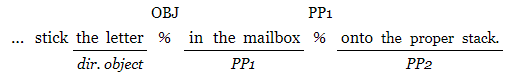
\includegraphics{breakpos.png}

Please work with the assumption that ``prosodic boundary'' in what follows is any subset of the following features, clustered in such a way as to trigger your intuition that a new prosodic element (of any size) is beginning: pitch change, volume change, segmental lengthening, or pause.

\begin{itemize}
\tightlist
\item
  Break after V?: Please indicate whether or not you think there is a prosodic boundary after the verb cluster(at the right edge of the last/main verb).
\item
  Break after OBJ?: Please indicate whether or not you think there is a prosodic boundary after the first NP in the object region (at the right edge of the first NP in the object region).
\item
  Break after PP1?: Please indicate whether or not you think there is a prosodic boundary after the first NP in the PP1 region (at the right edge of the first NP in the PP region).
\item
  Strongest break? Please indicate which of the breaks (columns E-G where you indicated YES) you think is strongest. If two breaks are of equal strength and are stronger than a third, indicate NONE as strongest. If two breaks are of equal strength and are weaker than a third, indicate that third break as strongest. If all breaks are the same strength, indicate NONE as strongest.
\item
  Weakest break? Please indicate which of the breaks (columns E-G where you indicated YES) you think is weakest. If two breaks are of equal strength and are weaker than a third, indicate NONE as weakest. If two breaks are of equal strength and are stronger than a third, indicate that third break as weakest. If all breaks are the same strength, indicate NONE as weakest
\item
  Struggle?: Indicate whether or not the speaker appears to have had difficulty reading the sentence. This should be relative to their baseline reading fluency, so if a person is hesitant every time, hesitance should not be enough to indicate a struggle.
\item
  Start of struggle: indicate the region in which you first notice the speaker struggling.
  *Question?: indicate simply whether or not the recording sounds like a question, prosodically (e.g., final rise is present).
\end{itemize}

\clearpage

\hypertarget{references}{%
\chapter*{References}\label{references}}
\addcontentsline{toc}{chapter}{References}

\noindent
\vspace{-2em}
\setlength{\parindent}{-0.5in}
\setlength{\leftskip}{0.5in}
\setlength{\parskip}{15pt}
\onehalfspacing

\hypertarget{refs}{}
\leavevmode\hypertarget{ref-ashby2012eye}{}%
Ashby, J., Yang, J., Evans, K. H., \& Rayner, K. (2012). Eye movements and the perceptual span in silent and oral reading. \emph{Attention, Perception, and Psychophysics}, \emph{74}(4), 634--640.

\leavevmode\hypertarget{ref-Bader1998-ts}{}%
Bader, M. (1998). Prosodic influences on reading syntactically ambiguous sentences. In \emph{Reanalysis in sentence processing} (pp. 1--46). Springer.

\leavevmode\hypertarget{ref-R-lme4}{}%
Bates, D., Maechler, M., Bolker, B., \& Walker, S. (2019). \emph{Lme4: Linear mixed-effects models using 'eigen' and s4}. Retrieved from \url{https://CRAN.R-project.org/package=lme4}

\leavevmode\hypertarget{ref-Beckman1997-eu}{}%
Beckman, M. E., \& Ayers, G. (1997). Guidelines for ToBI labelling. \emph{The OSU Research Foundation}, \emph{3}, 30.

\leavevmode\hypertarget{ref-bever1970}{}%
Bever, T. G. (1970). The cognitive basis for linguistic structures. \emph{Cognition and the Development of Language}, \emph{279}(362), 1--61.

\leavevmode\hypertarget{ref-chomsky2014minimalist}{}%
Chomsky, N. (2014). \emph{The minimalist program}. MIT press.

\leavevmode\hypertarget{ref-clifton1988restrictions}{}%
Clifton, C., Jr. (1988). Restrictions on late closure: Appearance and reality. \emph{6th australian language and speech conference}, 19--21.

\leavevmode\hypertarget{ref-cliftonEtAl1991}{}%
Clifton, C., Jr., Speer, S., \& Abney, S. P. (1991). Parsing arguments: Phrase structure and argument structure as determinants of initial parsing decisions. \emph{Journal of Memory and Language}, \emph{30}(2), 251--271.

\leavevmode\hypertarget{ref-Cuetos1988-tm}{}%
Cuetos, F., \& Mitchell, D. C. (1988). Cross-linguistic differences in parsing: Restrictions on the use of the late closure strategy in spanish. \emph{Cognition}, \emph{30}(1), 73--105.

\leavevmode\hypertarget{ref-den2006relators}{}%
Den Dikken, M. (2006). \emph{Relators and linkers: The syntax of predication, predicate inversion, and copulas} (Vol. 47). MIT press.

\leavevmode\hypertarget{ref-gmm1}{}%
Falk, T. H., \& Chan, W.-Y. (2006). Nonintrusive speech quality estimation using gaussian mixture models. \emph{IEEE Signal Processing Letters}, \emph{13}(2), 108--111.

\leavevmode\hypertarget{ref-Fodor2002-io}{}%
Fodor, J. D. (2002). Psycholinguistics cannot escape prosody. \emph{Speech prosody 2002, international conference}.

\leavevmode\hypertarget{ref-fodor2019center}{}%
Fodor, J. D., Macaulay, B., Ronkos, D., Callahan, T., \& Peckenpaugh, T. (2019). Center-embedded sentences: An online problem or deeper? In \emph{Grammatical approaches to language processing} (pp. 11--28). Springer.

\leavevmode\hypertarget{ref-Frazier1979-pb}{}%
Frazier, L. (1979). \emph{On comprehending sentences: Syntactic parsing strategies}.

\leavevmode\hypertarget{ref-frazier1996construal}{}%
Frazier, L., \& Clifton, C., Jr. (1996). \emph{Construal}. MIT Press.

\leavevmode\hypertarget{ref-frazier1978sausage}{}%
Frazier, L., \& Fodor, J. D. (1978). The sausage machine: A new two-stage parsing model. \emph{Cognition}, \emph{6}(4), 291--325.

\leavevmode\hypertarget{ref-goldman1961-pa}{}%
Goldman-Eisler, F. (1961). The distribution of pause durations in speech. \emph{Language and Speech}, \emph{4}(4), 232--237.

\leavevmode\hypertarget{ref-Hedberg2017-er}{}%
Hedberg, N., Sosa, J. M., \& Görgülü, E. (2017). The meaning of intonation in yes-no questions in american english: A corpus study.

\leavevmode\hypertarget{ref-jacewicz2010-sr}{}%
Jacewicz, E., Fox, R. A., \& Wei, L. (2010). Between-speaker and within-speaker variation in speech tempo of american english. \emph{The Journal of the Acoustical Society of America}, \emph{128}(2), 839--850.

\leavevmode\hypertarget{ref-kimball1973seven}{}%
Kimball, J. (1973). Seven principles of surface structure parsing in natural language. \emph{Cognition}, \emph{2}(1), 15--47.

\leavevmode\hypertarget{ref-Kjelgaard1999-xd}{}%
Kjelgaard, M. M., \& Speer, S. R. (1999). Prosodic facilitation and interference in the resolution of temporary syntactic closure ambiguity.

\leavevmode\hypertarget{ref-R-lmerTest}{}%
Kuznetsova, A., Bruun Brockhoff, P., \& Haubo Bojesen Christensen, R. (2019). \emph{LmerTest: Tests in linear mixed effects models}. Retrieved from \url{https://CRAN.R-project.org/package=lmerTest}

\leavevmode\hypertarget{ref-evs}{}%
Laubrock, J., \& Kliegl, R. (2015). The eye-voice span during reading aloud. \emph{Frontiers in Psychology}, \emph{6}(1432). \url{https://doi.org/10.3389/fpsyg.2015.01432}

\leavevmode\hypertarget{ref-os2012}{}%
Mathôt, S., Schreij, D., \& Theeuwes, J. (2012). OpenSesame: An open-source, graphical experiment builder for the social sciences. \emph{Behavior Research Methods}, \emph{44}(2), 314--324. \url{https://doi.org/10.3758/s13428-011-0168-7}

\leavevmode\hypertarget{ref-mehler1963some}{}%
Mehler, J. (1963). Some effects of grammatical transformations on the recall of english sentences. \emph{Journal of Verbal Learning and Verbal Behavior}, \emph{2}(4), 346--351.

\leavevmode\hypertarget{ref-qp2}{}%
Peckenpaugh, T. (2016). \emph{Interrogative context and PP-attachment ambiguities}.

\leavevmode\hypertarget{ref-Prince1993-ic}{}%
Prince, A., \& Smolensky, P. (1993). Optimality theory: Constraint interaction in generative grammar.

\leavevmode\hypertarget{ref-raynerEtAl1983}{}%
Rayner, K., Carlson, M., \& Frazier, L. (1983). The interaction of syntax and semantics during sentence processing: Eye movements in the analysis of semantically biased sentences. \emph{Journal of Verbal Learning and Verbal Behavior}, \emph{22}(3), 358--374.

\leavevmode\hypertarget{ref-rayner2012psychology}{}%
Rayner, K., Pollatsek, A., Ashby, J., \& Clifton, C., Jr. (2012). \emph{Psychology of reading}. Psychology Press.

\leavevmode\hypertarget{ref-salverda2003role}{}%
Salverda, A. P., Dahan, D., \& McQueen, J. M. (2003). The role of prosodic boundaries in the resolution of lexical embedding in speech comprehension. \emph{Cognition}, \emph{90}(1), 51--89.

\leavevmode\hypertarget{ref-schafer2000intonational}{}%
Schafer, A. J., Speer, S. R., Warren, P., \& White, S. D. (2000). Intonational disambiguation in sentence production and comprehension. \emph{Journal of Psycholinguistic Research}, \emph{29}(2), 169--182.

\leavevmode\hypertarget{ref-Selkirk1986-hc}{}%
Selkirk, E. O. (1986). \emph{Phonology and syntax: The relation between sound and structure}. MIT Press (MA).

\leavevmode\hypertarget{ref-selkirk2011-hp}{}%
Selkirk, E. O. (2011). The syntax-phonology interface. In J. Goldsmith, J. Riggle, \& A. Yu (Eds.), \emph{The handbook of phonological theory} (Vol. 2, pp. 435--483). Oxford: Blackwell Publishing.

\leavevmode\hypertarget{ref-p600addscps}{}%
Steinhauer, K. (2003). Electrophysiological correlates of prosody and punctuation. \emph{Brain and Language}, \emph{86}(1), 142--164.

\leavevmode\hypertarget{ref-streeter1978acoustic}{}%
Streeter, L. A. (1978). Acoustic determinants of phrase boundary perception. \emph{The Journal of the Acoustical Society of America}, \emph{64}(6), 1582--1592.

\leavevmode\hypertarget{ref-Truckenbrodt1999-vd}{}%
Truckenbrodt, H. (1999). On the relation between syntactic phrases and phonological phrases.

\leavevmode\hypertarget{ref-wax1985detection}{}%
Wax, M., \& Kailath, T. (1985). Detection of signals by information theoretic criteria. \emph{IEEE Transactions on Acoustics, Speech, and Signal Processing}, \emph{33}(2), 387--392.


\end{document}
